\chapter{NOTEBOOKS FROM TRASHED PAPERS}



\begin{singlespace}
\epigraph{The first question I ask myself when something doesn’t seem to be beautiful is why do I think it’s not beautiful? And very shortly you discover that there is no reason. If we can conquer that dislike, or begin to like what we did dislike, then the world is more open. That path ---of increasing one’s enjoyment of life--- is the path, I think, we all best take: to use art not as self-expression, but as self-alteration; to become more open.}{\hfill---John Cage, \textit{Wild Art}, 2013}
\end{singlespace}



In this chapter thesis project and its development progress will be explained in detail in the light of what has been discussed in previous chapters. The project will be examined in various dimensions. The relationship will be established between the previously mentioned artworks and project. How this project is related to the discussed concepts and how it can be positioned among the previous works will be explained.

Firstly, I briefly state and describe my work. Secondly, the development of the project and experiments are explained. Lastly, the final body of the work with its parts is presented.



%****************************************
\section{The Statement}
Refuse is part of people’s consumption practices. It is a very common concept from urban areas to rural ones, from modern societies to ancient ones. It is not wanted, thrown away, kept away. It is considered as useless, disgusting, abject, unattractive, and harmful to the people and nature. Contrary to the common approach as \citet[7]{thompson1979rubbish}, author of the book \textit{Rubbish Theory}, stated \quotes{one man’s trash is another man’s treasure}.

With the collaboration of many people discarded papers and packages were collected from different places. This time, it was not thrown away, it was collected and saved. Later they were transformed to notebooks by hand with traditional methods. Juxtaposition of trashes create notebooks that are different from the blank industrial ones, and through them challenged the widespread understanding of trash.

Through this project, I put all my effort to re-imagine, re-consider and re-think trash for seeking new possibilities and alternatives. As it is discarded, missed potentials were discovered. Strictly speaking, this project aims to find new potentials on trash.

The purpose is not to build an object that is produced from discarded material in order to watch it from distance. The important thing is to interact with it. It is already discarded and general behavior is to avoid from it. This work must change it. It must call the viewer to interact with it. In other words, trash must be accepted by them. This project asks people to readmit the trash to the their life. For this reason notebooks are given away free at various places where people visit frequently. By doing that once thrown materials would find a place with new purposes in the community.



%****************************************
\section{Development Progress of the Project}
In order to have an insight of this project and realize artistic intentions, it is important to look at the process that reveals the path to the final work and critical decisions that were necessary to the completion of the project.

Through the process, there are several problems that needed to be solved. Some of the questions in my mind are solved through the research on the subject. Further, the found samples of artworks played significant role in progress. They helped me a lot to shape unclear points of the project. They provide me a deeper understanding of the subject and what I am doing. In other words, they lead me during the development of the work.



% NEW PART [approach, history] 
Before explaining the details of the work, it would be better to explain how it was started and what is my approach to the trash.

My interaction with discarded material is not limited with this thesis project. There are a few previous attempts and several memories that I remember. Briefly, I want to examine them. These will also reveal my motivation and approach shaped through time and how thesis work affected from it.

% [SODA CAPS]
I remember from my childhood that we were collecting soda caps and were playing with them. We were looking everywhere to collect them. Some caps were found less and they worth more in the game. We put them on the railways to make them flat. After the train had passed we had perfect flat caps for our games. At that time, it was not waste for us. It has a value and part of our games and indispensable source of fun. The notion of playing with it can be related with the Picasso’s collage work \textit{Still Life with Chair Caning} mentioned previously. He pasted letters of the French word \quotes{JOU} means \quotes{game} signifying that playing with the materials. We were already playing with trash while we were child. Therefore, it can be better understand that why Picasso said that \quotes{every child is an artist}.

% [VASVIYE HOCA]
Another important memory is from my primary school teacher. When I was at third class, our teacher wanted us to bring colorful papers to make something (whatever it is I do not remember now). The day after we brought some colorful paper that was bought from stationery store. Our papers’ shape and color looked same. However her papers were different in every dimension. They were cut out from packages and advertisements. I remember clearly that she suggested us to do the same: \quotes{Do not throw out packages, look for the useful parts and keep them to use later.} Whenever I am going to throw something away, this comes to my mind: Can it be reused? Every time it is not obvious that how can it be useful, but at some point it becomes an \quotes{indispensable practice.} Further, this practice also supports to the \textit{bricolage} methodology. Keeping many things makes easier to build (or produce) whatever at hand. 

% [Song Dong]
The main idea is to save them to use later. For some people it is a life saving practice. It can be seen in the case of artist Song Dong’s mother (mentioned in chapter 2). This practice result in establishing stronger and intimate relationship with objects. 

I am very uncomfortable with the act of discarding. I often think that by discarding objects, I am missing their potentials. I must find another use which is more effective than throwing away. At least I can give them to someone else who can use it for own purposes. Seeing papers on the waste bin is a disappointment for me. As artist Aaron Kramer argues and I strongly agree with that \quotes{[t]rash is the failure of imagination} \citep[as cited in][16]{meyer2007turning}. There is a lot of effort to produce objects and it seems that all this efforts are wasted. What I mention is not related about ultimate productivity. It is more close to being thoughtful, and taking responsibility of tools, items and objects that we are using. Rather than throwing out, creating a way that all are have chance to live together is much more close to my perception. On the contrary, sometimes I became overwhelmed because of the significant amount of leftover from daily activities and in order to move on I need to leave them behind. It is the result of inevitable rhythm of modern life style. Consuming and wasting is part of people’s daily routine and most of the time they are not aware of what they consume, and what they discard. In the scope of this thesis subject, saving objects rather them getting rid of them is an effective way of breaking the routines. The usage of that object can be decided in the future. 

% [encouraging point]
One of the encouraging factor of working on trash is to explore something different that others cannot see. In other words, it contains eureka moments. Because it is ignored by discarding and therefore it has undiscovered potentials. It waits us to be discovered and possibly (as Picasso’s explanation on his work \textit{Bull’s Head}\footnote{See epigraph in the beginning of chapter 3}, 1942) discovered again and again. 

% [EXPERIMENTS AT HOME]
My remarkable interaction with trash is from recent years. Long years I stayed at dormitory during when I was high school and university while undergraduate. Dormitory is place that living spaces is shared with many people. Therefore there is a limited place for you and your possessions and there is no space for unused items. After I graduated from university I started living in a rented house. This gives me to opportunity to save the materials to use them later. My very first intention is to use them on my paintings. Instead of white blank canvas I have experimented with different surfaces and I have collected boxes and cart boards from my friends. My aim is to turn discard materials to the different things. Here are some of my previous works.

\begin{figure}
  \begin{subfigure}[b]{0.31\textwidth}
    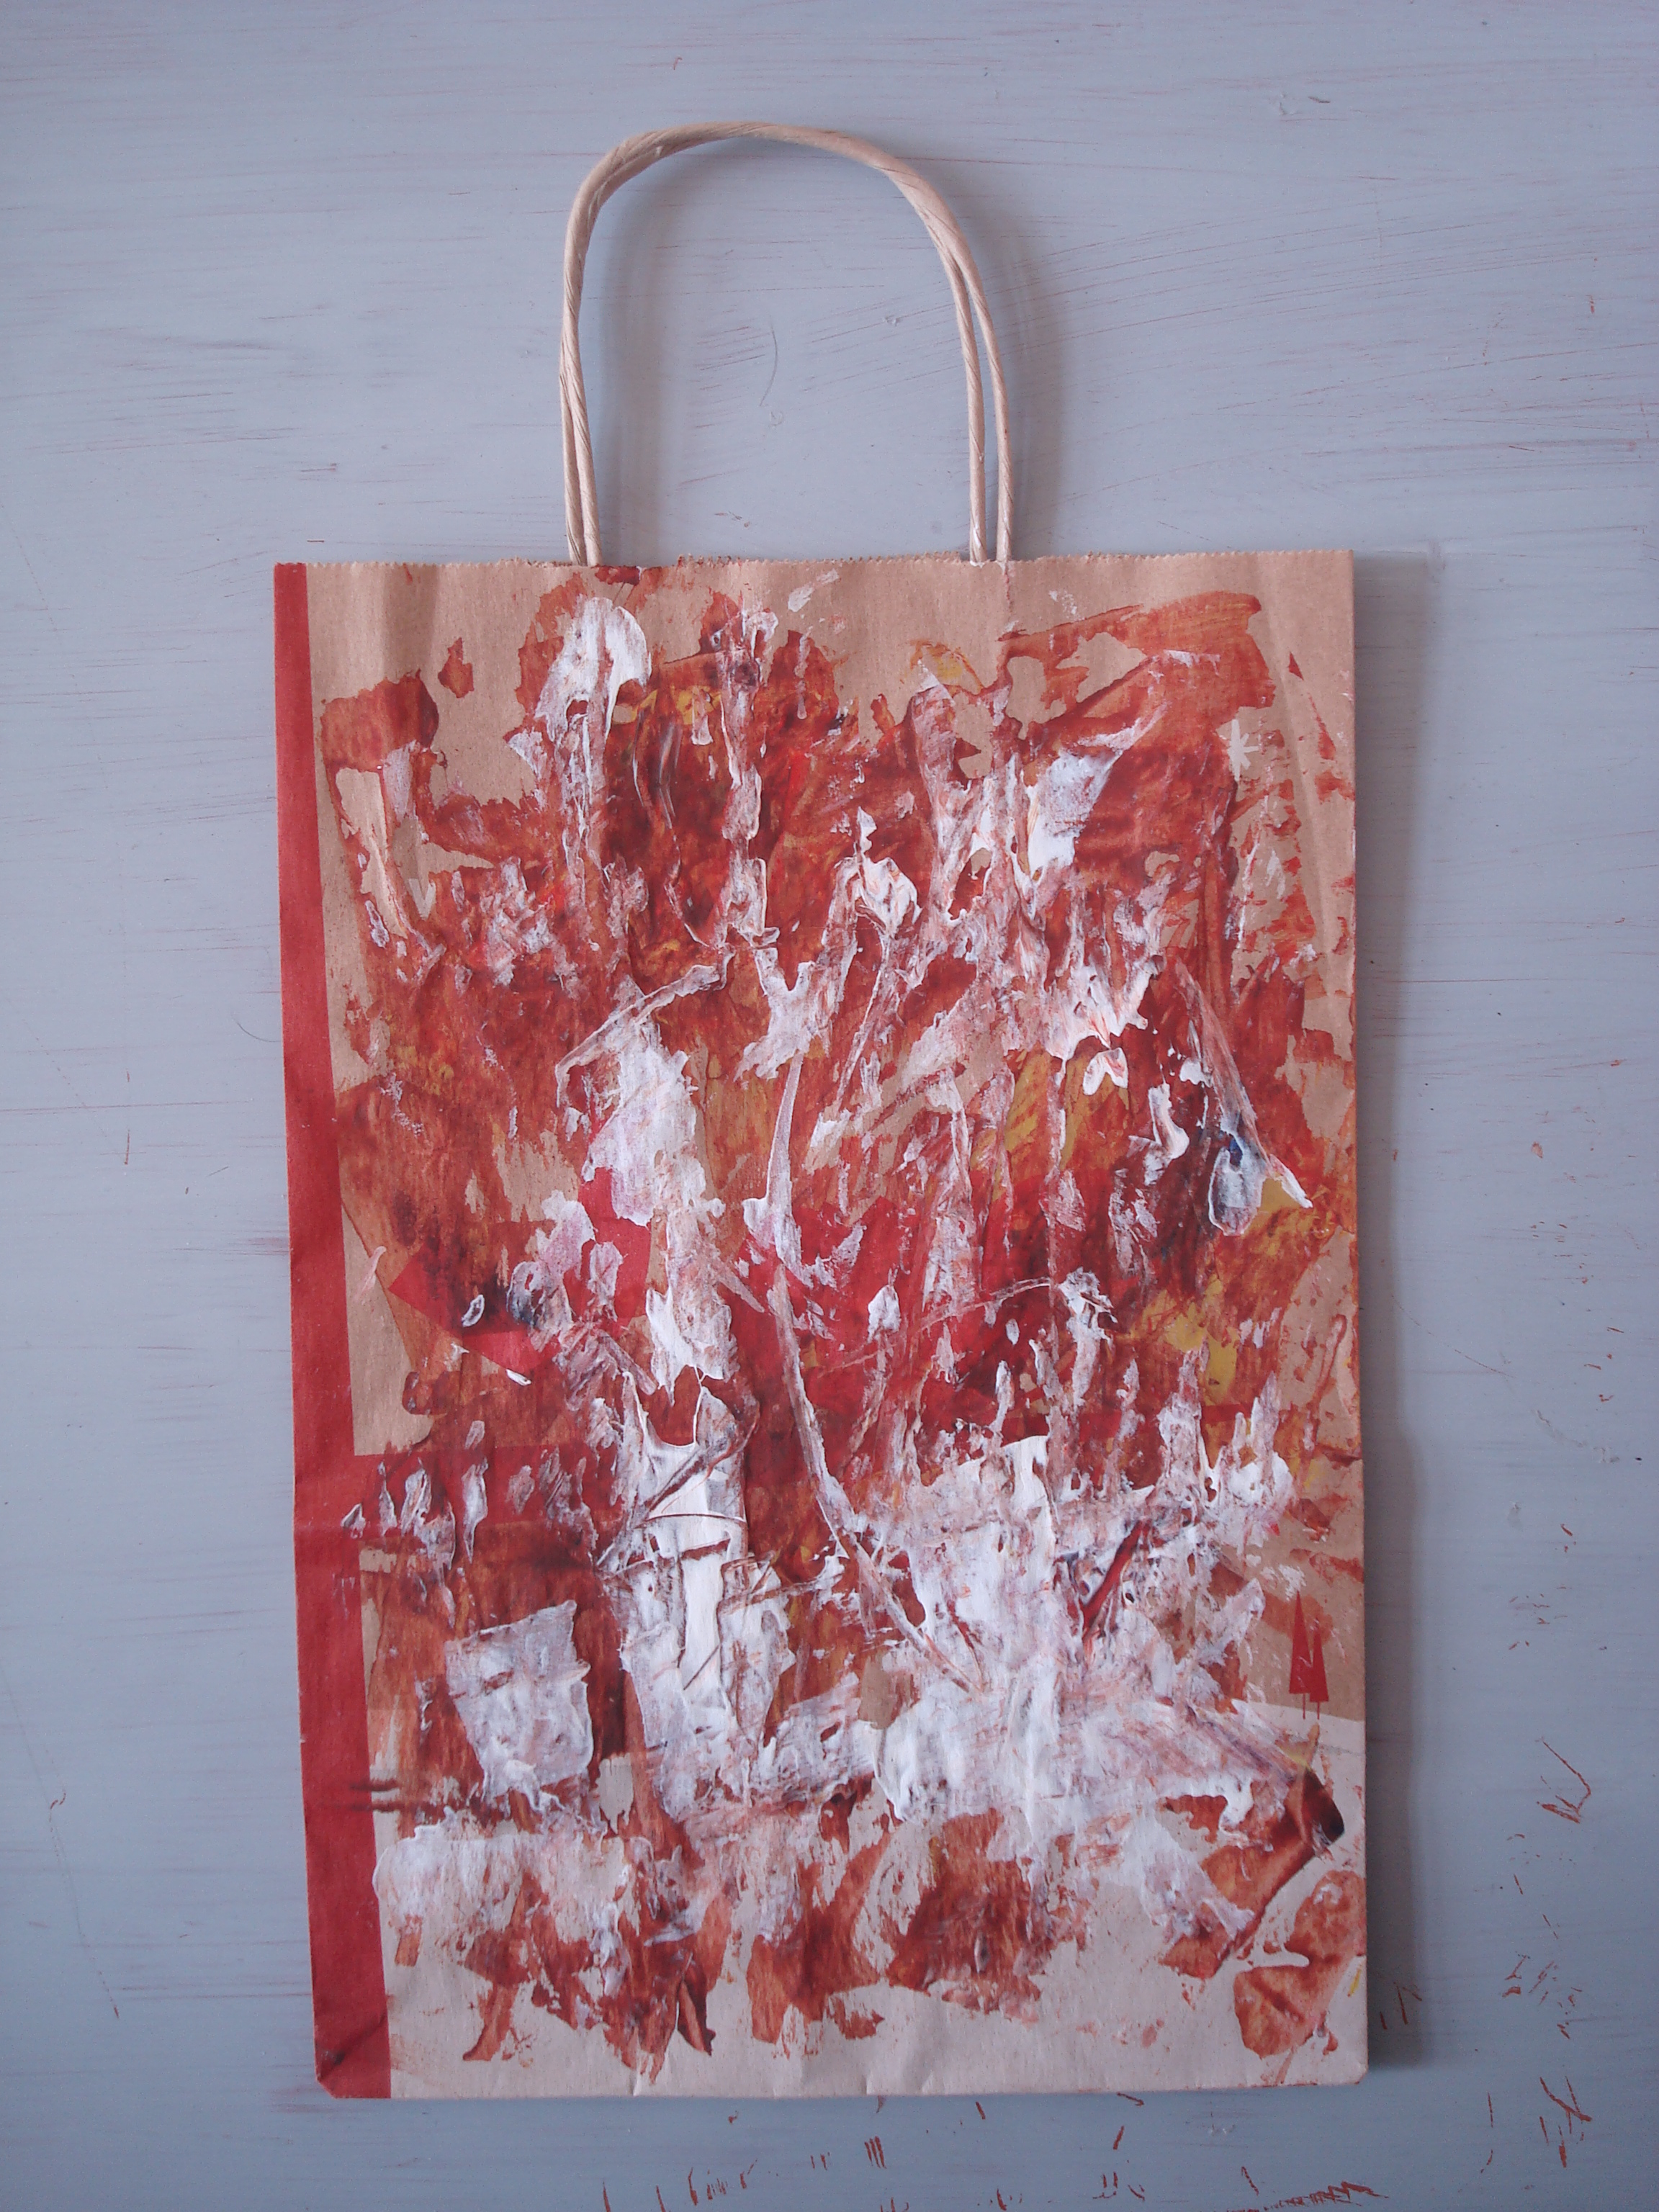
\includegraphics[width=\textwidth]{project_graphics/early_works1.jpg}
  \end{subfigure}
  \hfill
  \begin{subfigure}[b]{0.31\textwidth}
    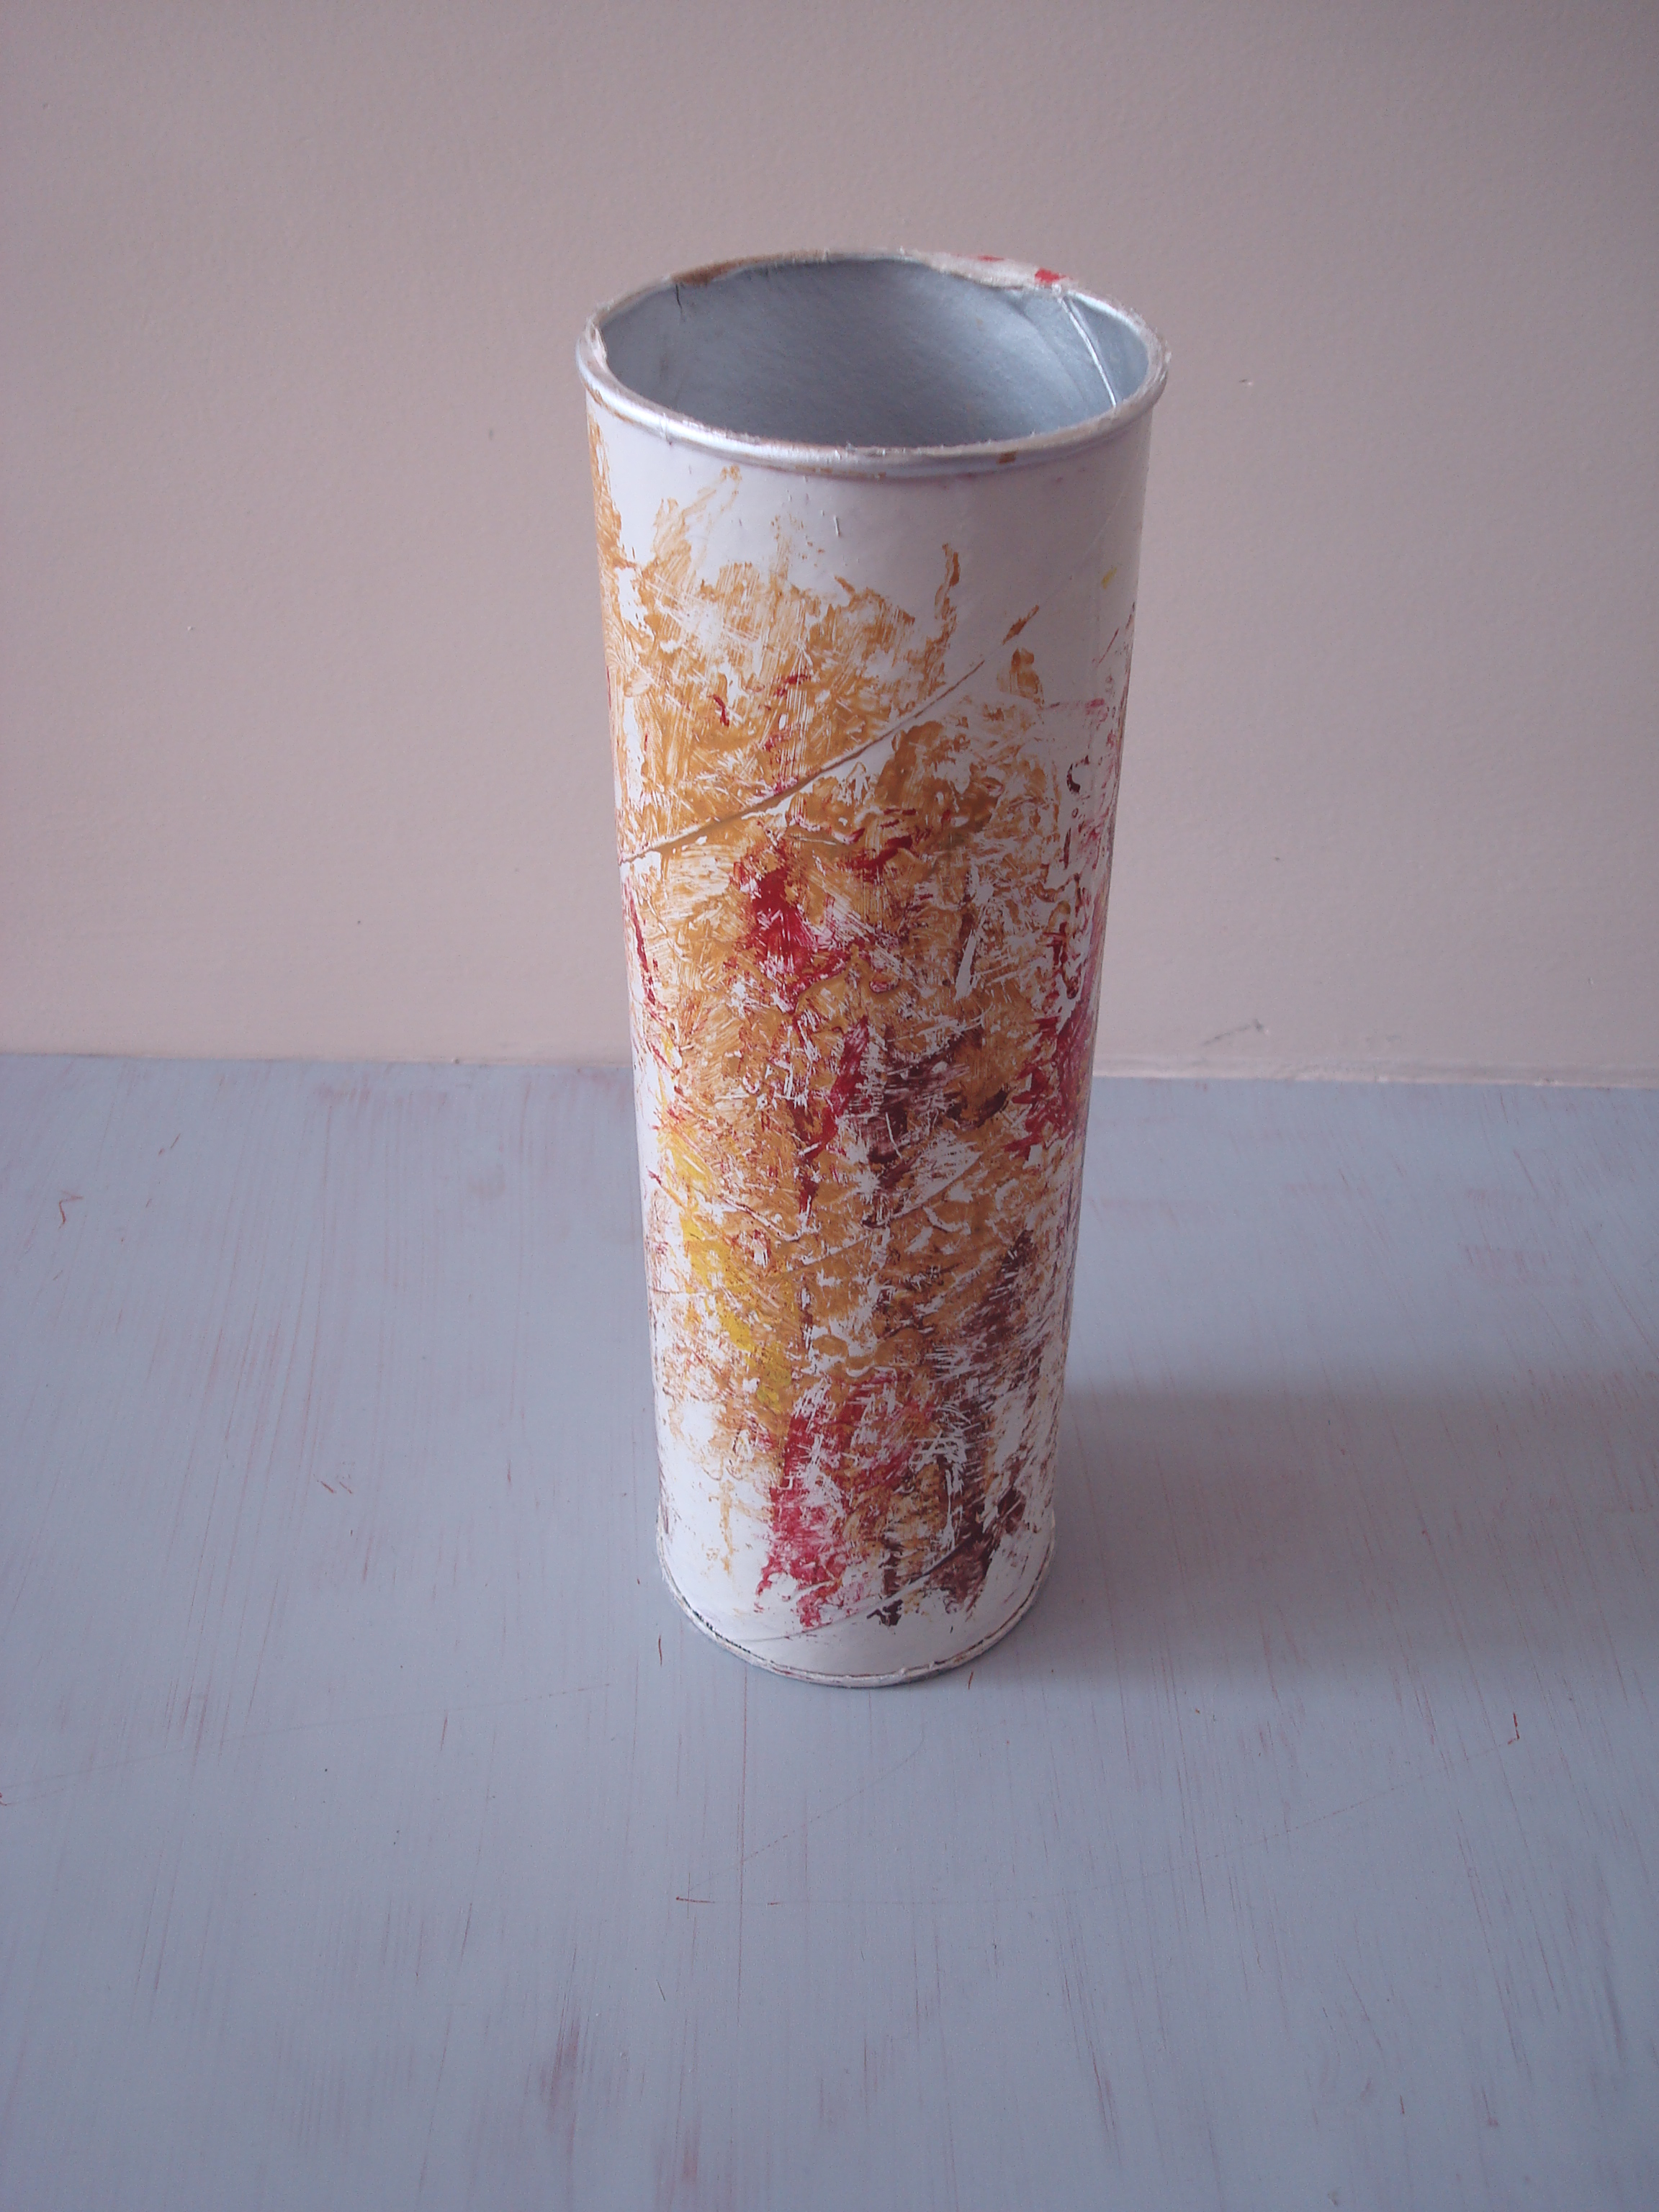
\includegraphics[width=\textwidth]{project_graphics/early_works2.jpg}
  \end{subfigure}
  \hfill
  \begin{subfigure}[b]{0.31\textwidth}
    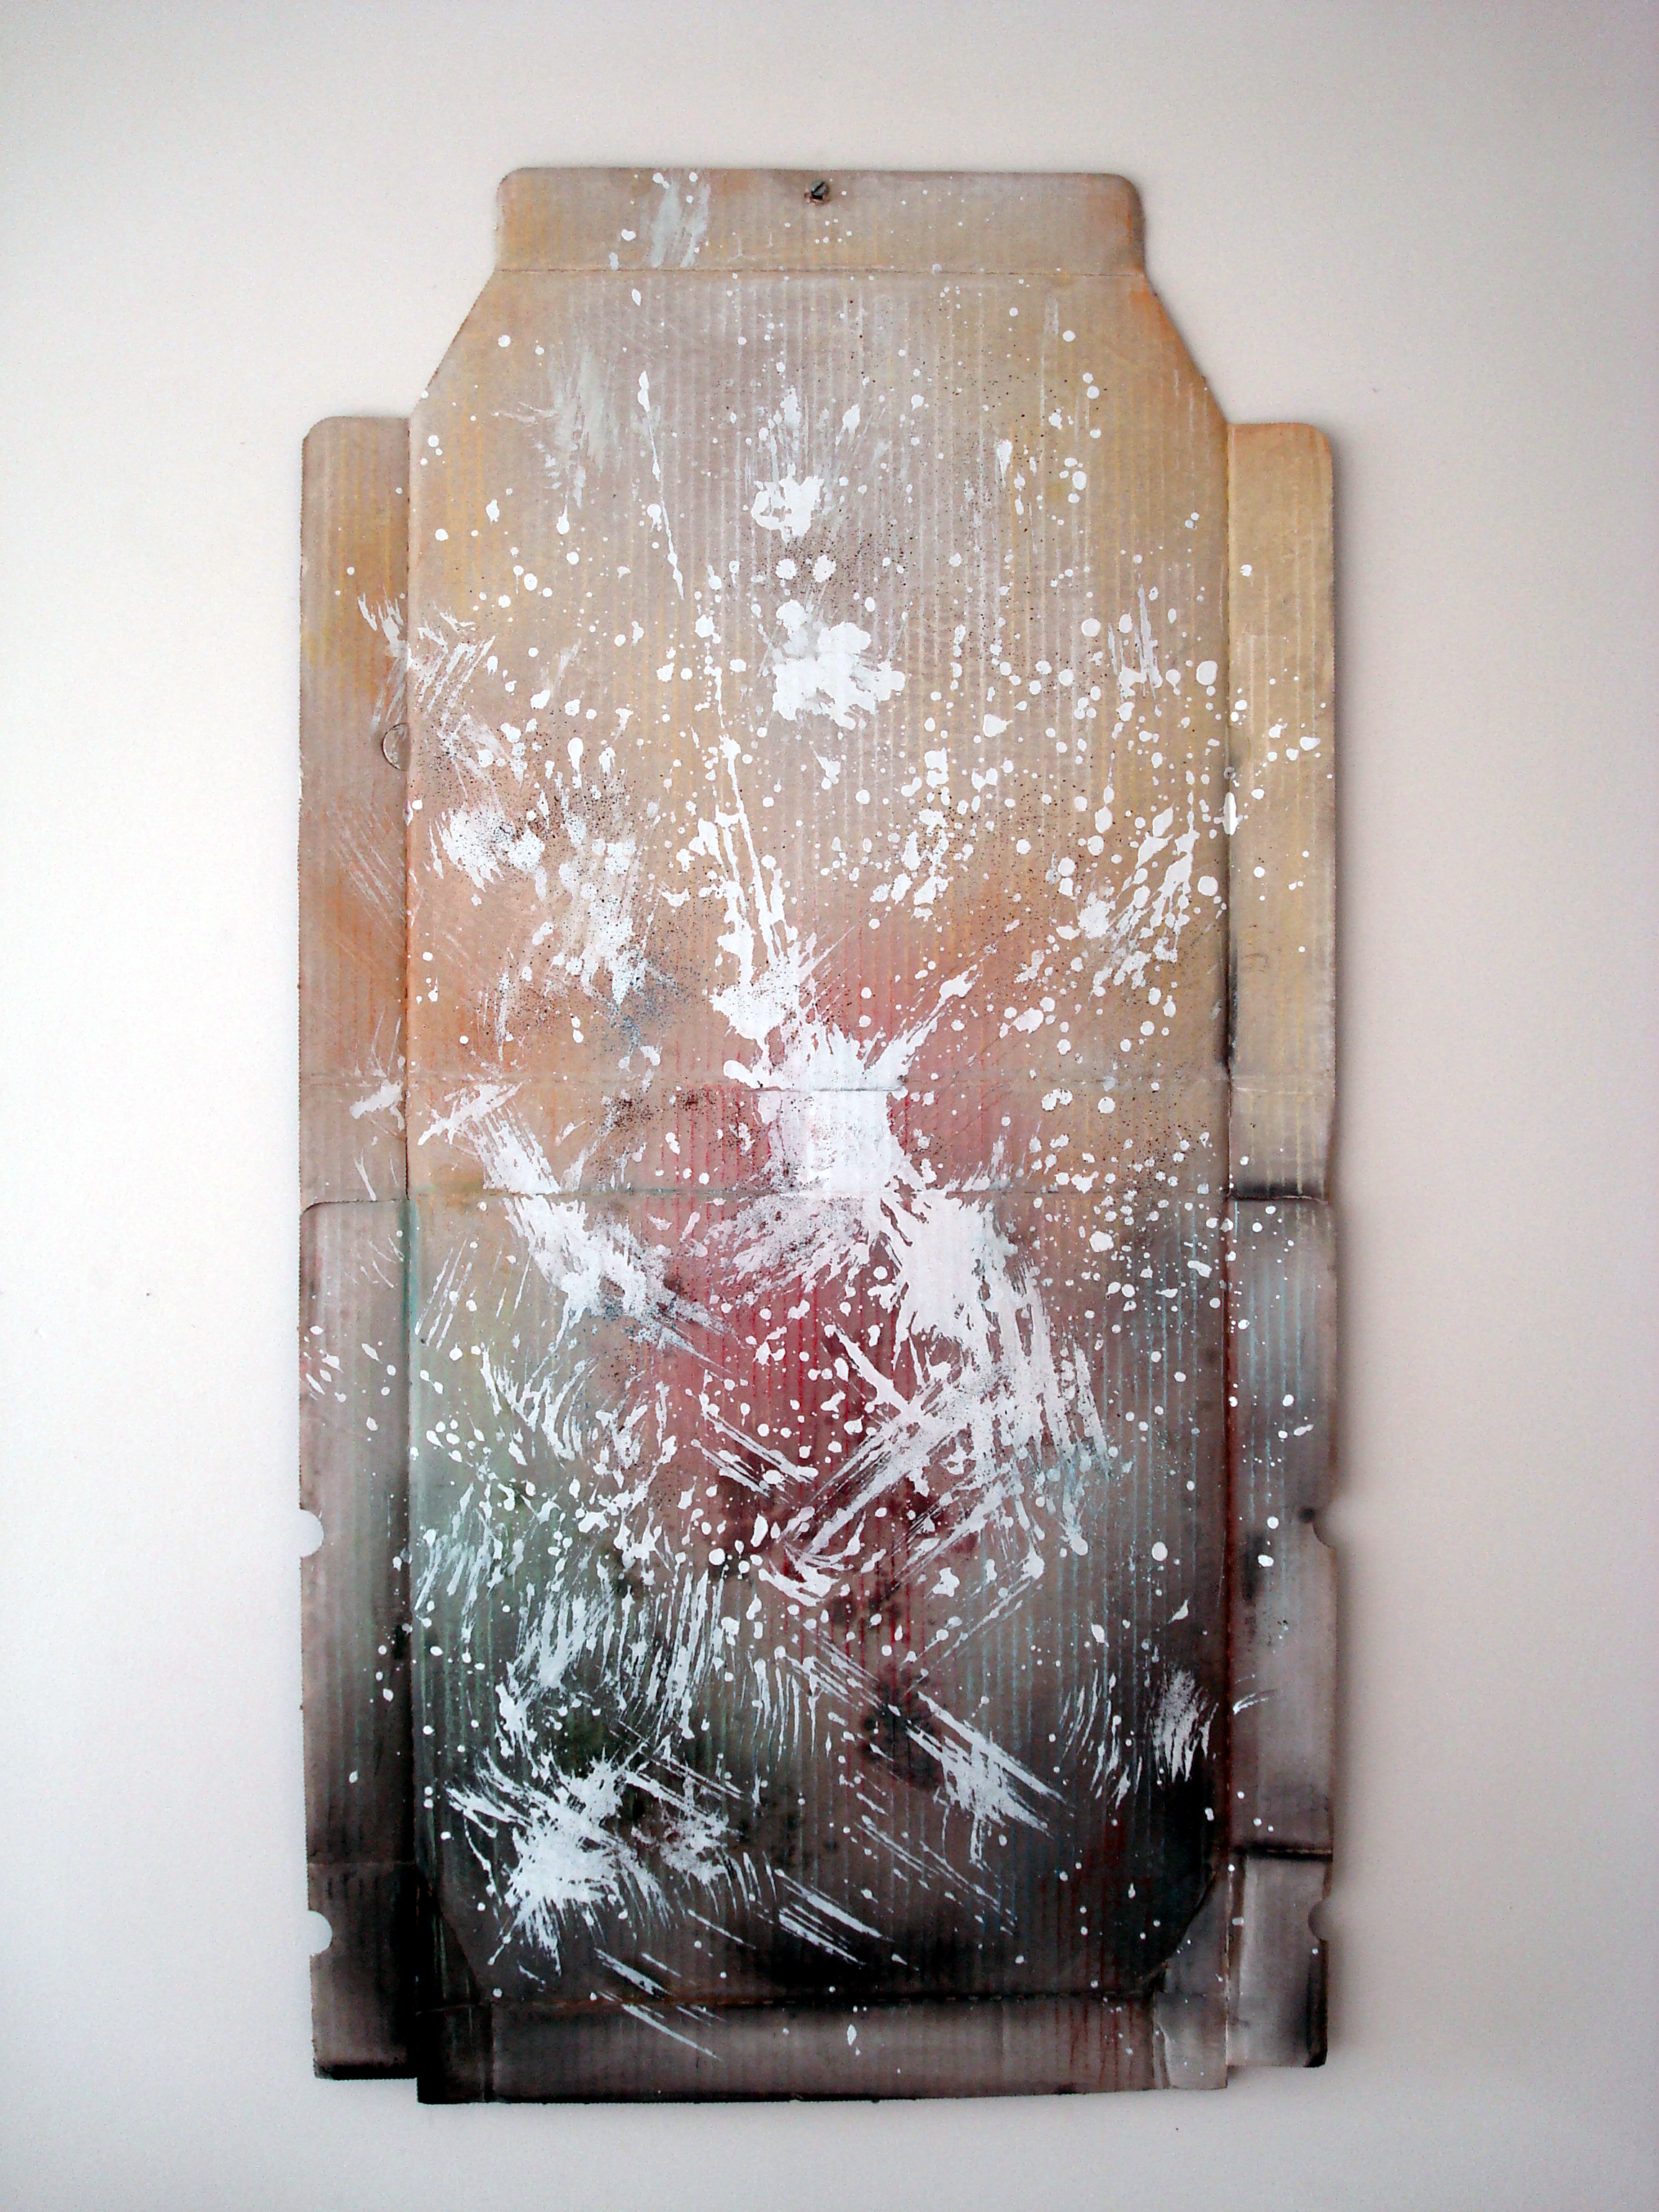
\includegraphics[width=\textwidth]{project_graphics/early_works3.jpg}
  \end{subfigure}
  \caption{Examples of early works}
  \label{fig:EarlyWorks}
\end{figure}

% TODO Free material add reference here.
My purpose in these work is to paint on different surfaces, experiment new materials. They are not flat, not blank. These surfaces bring their previous histories to the painting. Another factor is they are free and easily available. Therefore I can make many experiments on these materials. After I completed them, I showed them people around me and give them as a gift.

After turning discarded materials to different uses I began to collect them more eagerly. At the same time I also gave what I did to my friends as a birthday gift. I was experimenting with the material and at some point, with the help of my mother, I made my first notebook covered by a part of Starbucks bag. Papers inside of it are blank mimeograph paper which different than white paper. Particularly purpose is to move away from white paper because I feel uncomfortable when using it. It looks to me very bright. Therefore mimeograph paper is better for me. At that time it was a great victory for me. I started to carry it and use it every possible place. I show them to people and some of them supported to me giving their discard. One of them is my supervisor. He started to collect packages for me. After turning his packages to notebooks, he suggested me to go deeper in this subject and make my thesis project from them. Thereafter what I need is more discarded material.

% TODO Lars Eighner BIB’e eklenecek.



%****************************************
\subsection{Collecting}
Collecting discarded objects has carried out through the efforts of mine and people around me. Lars Eighner’s instructions helped me a lot when collecting objects. He writes that:

\begin{quote}
Eating safely from the Dumpsters involves three principles, using the senses and common sense to evaluate the condition of the found materials, knowing the Dumpsters of a given area and checking them regularly, and seeking always to answer the question \quotes{Why was this discarded?} \citep[as cited in][6]{strasser1999waste}.
\end{quote}

Does it discarded because of rotten, not fitting industrial standard or being production excess? For instance, in the documentary film of Agnés Varda, she records the potatoes that are discarded because of not fitting the industrial standards. Therefore these potatoes fall into the category of eatable.

I applied above instructions to my case and I checked discovered places regularly and seek the reason of why was it discarded. I also checked the condition of material. However I need to explore different locations to collect items. Most of them are not obvious for me. I discovered them on the flow of normal life and tasks. Similar to the methodology of Dick Jewell when searching for photos, my mode of search includes waste bins. However every object have a different story and they will be explained later.

Moreover there are other rules that define the frame of collecting act. Paper or package must be trash or will be trashed. For this project anything must not be intentionally bought to use as trash. In other words first rule is to consume less and generate less trash. Lots of trash is already produced every time everywhere. Aim is to reach them.

% OWNER
\quotes{The question of who owns these discards is not trivial} \citep{zimring2012encyclopedia}. This question makes me feel uncomfortable because of thinking that stealing that someone elses’ objects. Particularly I felt it when collecting left out papers from Bilkent Computer Laboratory. You already know that it owned by somebody else and after a while owner can take them. I solved this issue checking the leaved papers in every couples hours. If it stays there I take them. Further I encountered that If nobody takes them for a long time servants collect them.

The issue of owner becomes more complicated when owners’ social status considered. Zubiaurre mentions that no body cares her student scavenged through people’s trash in a poor neighborhood \citep[as cited in][]{pricano2011trashtalk}. On the contrary when the same student went to Beverly Hills home of the many actors and celebrities in California to scavenge nearly the police were called.

% CONTRIBUTIONS OF PEOPLE
As mentioned previously many people contributed to the project by collecting. Whenever I meet my friends I ask them to save their discard for the project. The importance of collaboration with them can be understood the term \quotes{citizen science} which is \quotes{defined as scientific research performed in part or in whole by volunteers who are not professional scientists} \citep{robson2012using}. I need to note that this is not a scientific project but the notion belongs there. The value of it lies in the collective intelligence of the contributors. In the scope of this thesis the term can be interpreted as people bring their own creativity and interpretation to the project by collecting the items that they reach and select. When the number of contributors are increased the diversity of the collected material will be increased and this will echo in the notebooks. 

It can be viewed as a co-authored work. Because many people helped me to collect the papers and also many people leave their trail to the paper and also they bring meaning to the them. After production of papers I also want them to continue as co-authored process. In other words many people will be part of this project. As people see different things on objects and bring them to me. the variety of things is increased in time. Because people said me that \quotes{I thought that you can use it. Do you collect also these?}. They bring their unique approach. 

They provide me the materials to transform it. They select the items and find them. They bring their approach and selection. They are part of the selection of the materials. They started to engage with the work. People bring the material also wonder the result of it. Further people see me when collecting objects and transporting them wonders their purpose. 

The purpose is here not only to transform objects but also change the perceptions of trash. Asking people to collect things and inform them started to shift in peoples mind.

Collected items reflect my and contributors’ consumption practices. People as mentioned previously consumption patterns can be tracked from their leftover. From logos of companies onto the packages reveal people’s choices and give clues about their social status.

% What type of activities generates waste.
Beyond social status it reveals activities that generate such a waste.It can be also extracted that most of the trashed papers are thrown away from feeding activity. On the other hand vastness of some types of disposables reveal the dark side of enterprises such as Starbucks and Burger King. Few people thought that after seeing the project I only collected Starbucks packets. There is no such a limitation but as a result of my habitat the number of them suppress the others.

%[disposable paper, packaging]
Collected items are mainly disposables ones. Most of them are paper or made from paper. The word paper comes from papyrus, the plant that was first used for writing in ancient Egypt long before the making of paper in China. In modern times all types and qualities of paper such as newspaper paper, print paper, and carton used for boxes pass through the same basic method of manufacture \citep{trafford2012paper}. It is fundamental medium for writing, reading, education, communication, information storage and many others. Its role in the development of human civilization can not be neglected. (Paper in several forms is consumed on a daily basis \citep{trafford2012paper}.) Wide range of use from packing to newspaper makes it indispensable product for people. On the other hand for artist it offers great diversity in order to make compositions as can be seen in the works of collage. Further it is easy to find and collect them. Even if it is thrown out, still appropriate for painting and writing.

Since paper is both biodegradable and a renewable resource, it is preferred by some of corporations for their products to show their respect to the nature. The motivation why they use can be seen their notes printed on the papers (Figure \ref{fig:NoteOnPackage}).

\begin{figure}[h!]
  \centering
  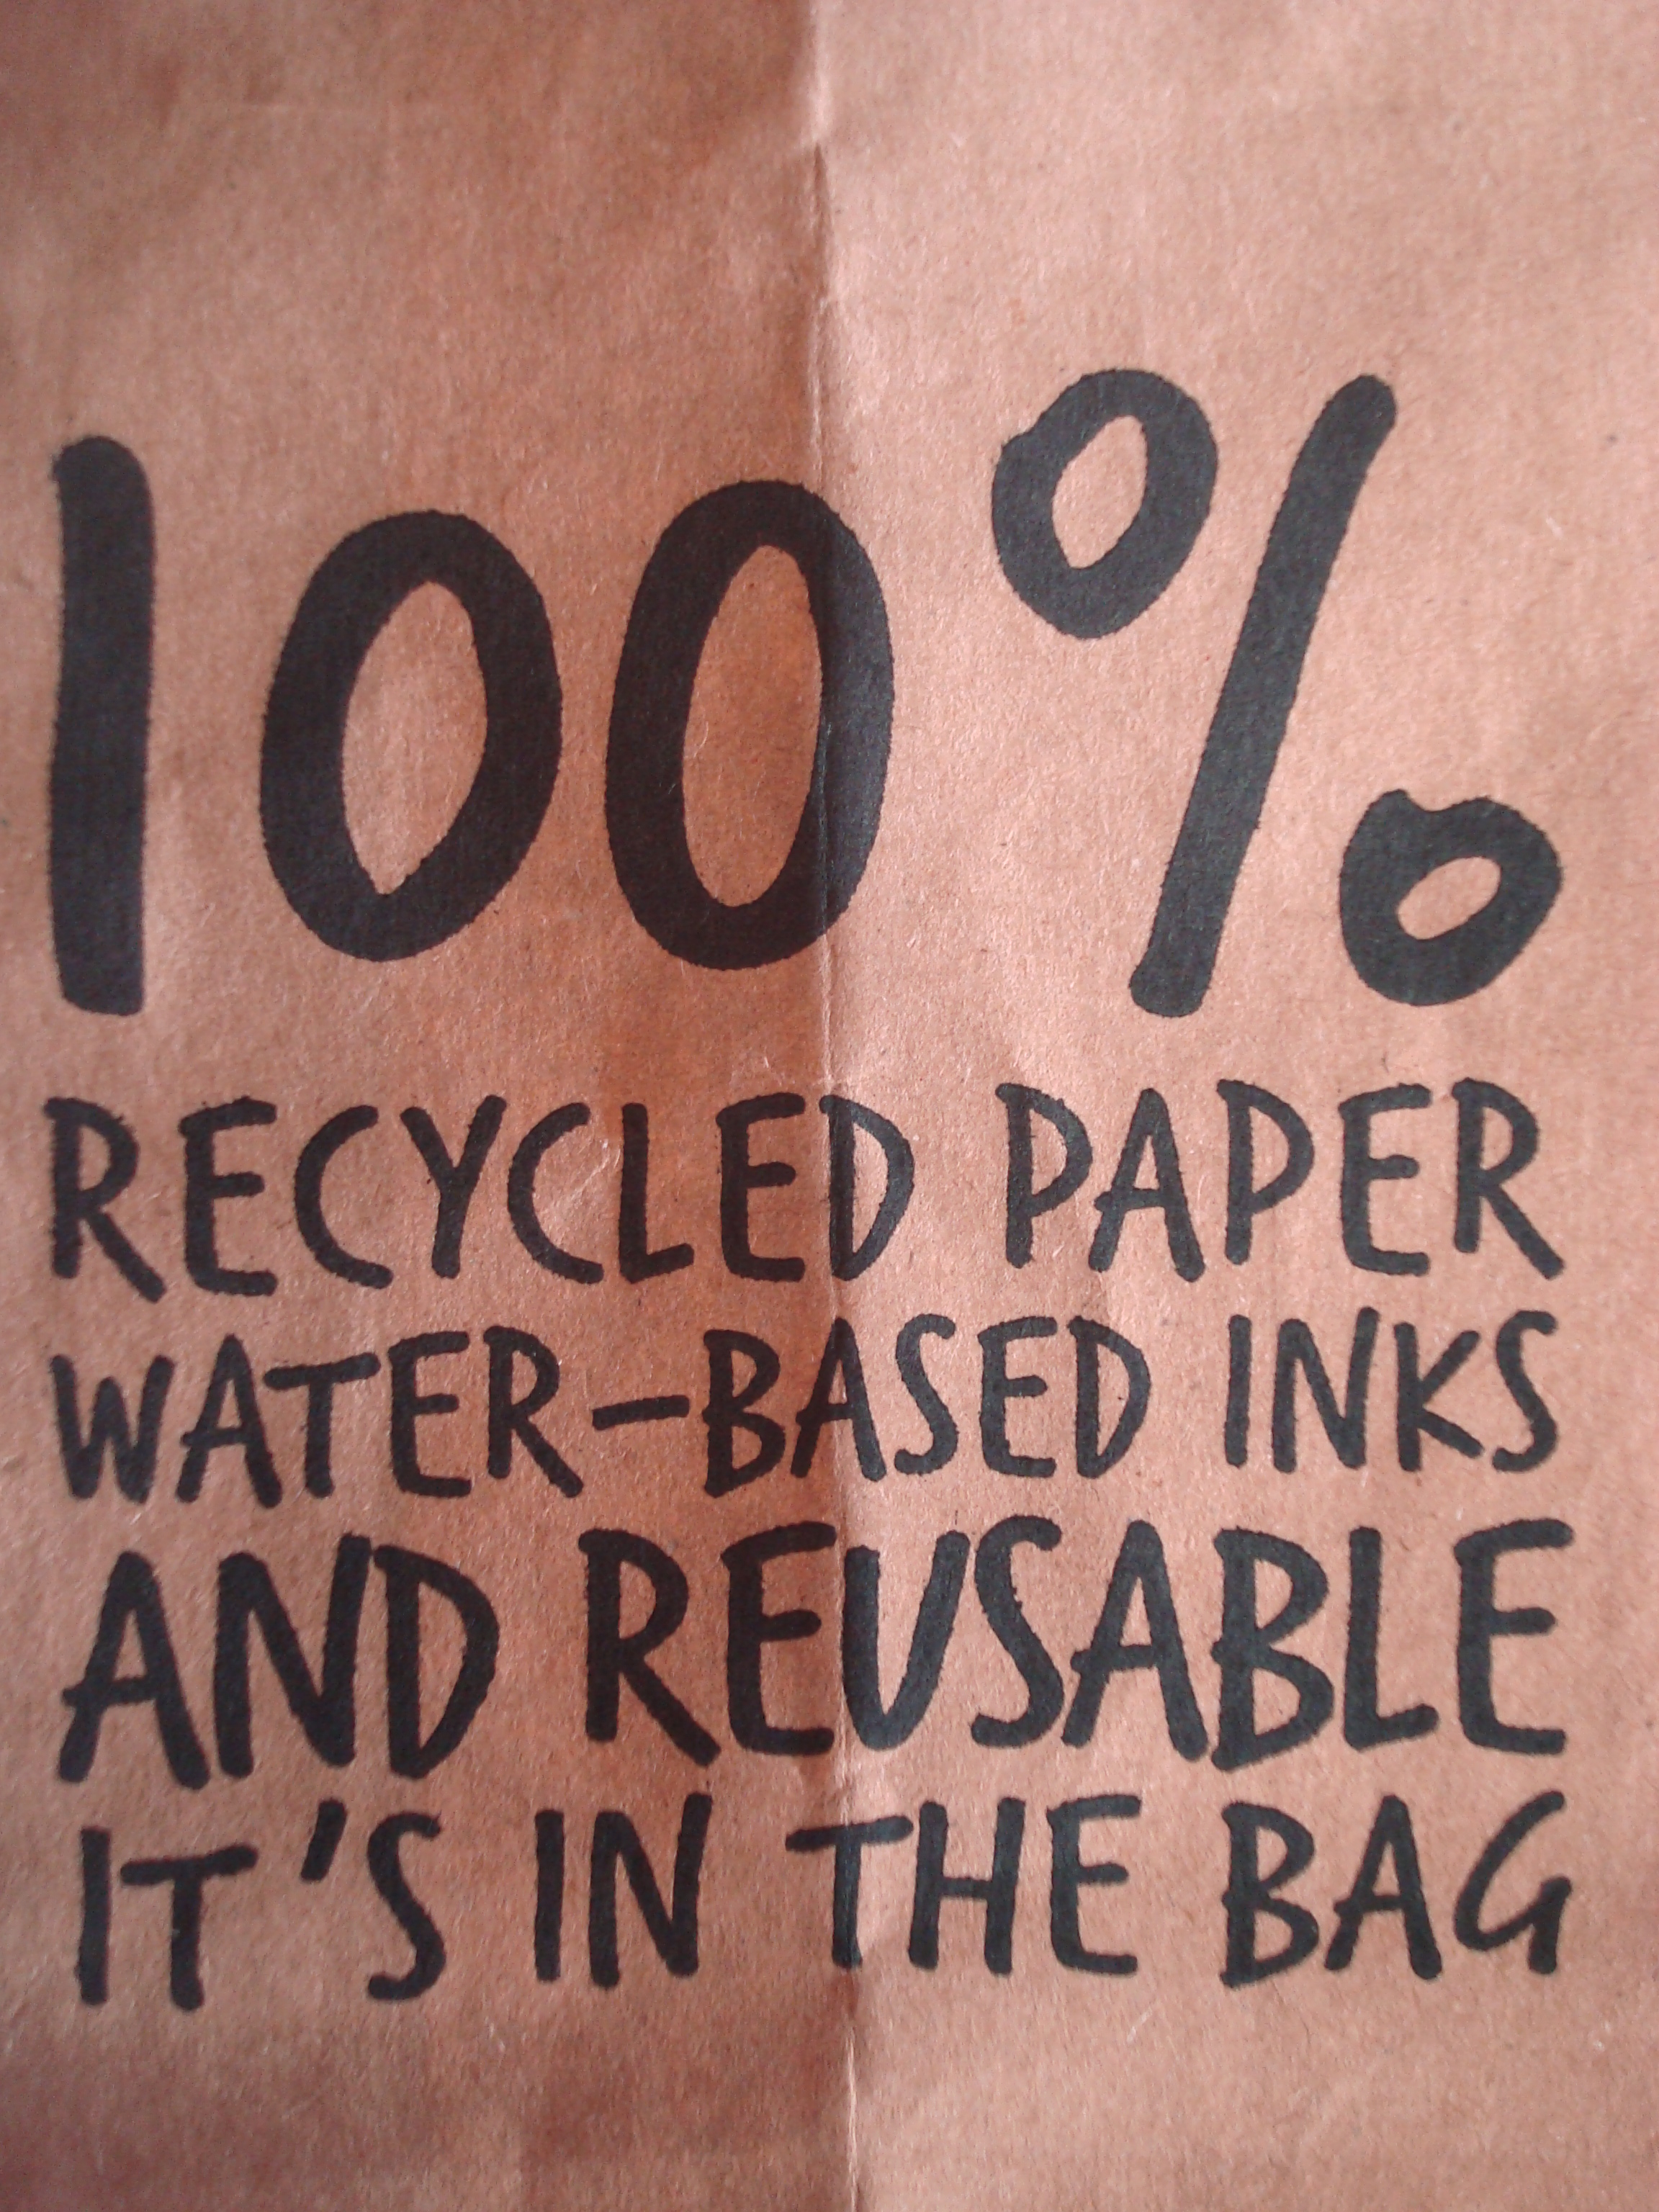
\includegraphics[height=6cm]{project_graphics/recycled_note.jpg}
  \caption{Recycling notice on the package}
  \label{fig:NoteOnPackage}
\end{figure}

The reason of collecting papers based on my interest on painting and writing. This medium offers me great possibilities that I cannot consume yet. This project is one of them.

Collected items (Figure \ref{fig:CollectedAllTogether}) are stored in my room for a long time. Most of them do not belong to me. Here the detailed information of the collected materials including the place where it is collected and their previous usage are listed.

\textbf{Burger King packages} (Figure \ref{fig:BurgerKingBag}) are collected from the office where I work. At lunch time, some of the colleagues order their meal from Burger King which is a global chain of fast food restaurant. Meals are delivered to the office with paper packages. The package of the meal is collected and used as a cover of notebooks. 

Inside the bag one paper package is used for French fries which is oily and paper is very good to absorb oil. Some people think that it is disgusting to use it for other purposes because of oil onto it. But immediately I replied them \quotes{you just eat that oily fires so what is wrong with it?} At the same time, what \citet[5]{strasser1999waste} said comes to my mind; \quotes{Nothing is inherently trash}. She refers to resolution on dirt of \citet[36]{douglas2003purity}:

\begin{quote}
Shoes are not dirty in themselves, but it is dirty to place them on the dining table; food is not dirty in itself but it is dirty to leave cooking utensils in the bedroom, or food bespattered on clothing; similarly bathroom equipment in the drawing room; clothing lying on chairs; out-door things in-doors; upstairs things downstairs; under-clothing appearing where over-clothing should be and so on.
\end{quote}

This simply explains that our perceptions to the objects which are relative and change in their usage context. Further it signifies that trash only catches attention of people when it is in wrong place. \citet[92]{thompson1979rubbish} argues that people only recognize rubbish when it is in unusual place and condition. He also points out rubbish in the wrong place is \quotes{emphatically visible and extremely embarrassing.} \citet[391]{parsons2008thompsons} concludes that rubbish is \quotes{no longer used or loved or cared for and often no longer seen. Rubbish objects linger on the periphery of our lives, in the back of the drawer, bottom of the wardrobe or cupboard, corner of the garage or garden shed gathering dust.}

\textbf{Starbucks packages} (Figure \ref{fig:StarbucksBag}) are collected from my supervisor, office where I work and my friend. Particularly my friend saved and collected them from her friends. Few of them collected from waste bins. They are used as a cover of notebooks. There are different types of packets from this category. As claimed by the company all of them are built from recycled ---precisely downcycled--- paper. There is also one category of object that is not paper. It is package of coffee beans. It is airtight and waterproof. It is very solid and strong. It has well graphic designs with different color and illustration.

\textbf{Modshifters papers} (Figure \ref{fig:Modshifters}) are used to cover the dinner table. Beginning of the table there is a big roll of paper to cover the table. At the end of the day used parts are cut out and thrown away. One of my visit I stayed there at a late time and catch the waiter when collecting the used papers and preparing tables to the next customer. I asked kindly him to give me these papers and he accepted. They are used as a cover of notebooks. All of them contains track of people who sit down there. I do not know any of them and I am not sure that the paper that they are laid down on their dinner turned to such a thing.

\textbf{Varuna Gezgin papers} (Figure \ref{fig:VarunaGezgin}) are the pages of obsolete dinner menu. When leaving there I showed my notebooks and asked to the cashier that I could able to present them at Varuna Gezgin. He immediately mentioned their vast amount of unused papers and gave me some of them that I can able to carry with me. This was a very strange experience for me because I did not expect such a thing. These paper are used inside of the notebooks as a page.

\textbf{The banner} (Figure \ref{fig:Banner_1}) is carried at graduation ceremony of Middle East Technical University in 2011 by the new Computer Engineering graduates. In Middle East Technical University there is a tradition that in graduation ceremony new grads walk through in the stadium and greet to the tribunes. With this event they carry some banners to express their feelings and point out the issues of the country in an ironic and humorous way. This one of them. At that time there are serious debates about freedom on the web. Most of the website are banned from the decision to the courts and they were not accessible. The slogan (Access to this banner is blocked by a court decision) decided by the new grads and before the ceremony I printed out the slogan to carried out as many people as it can and easy to readable from the people who seat at the tribunes.After the ceremony I could not throw away this banner. I do not know what to do it. It is a very big roll of paper to save but I could not throw away. I think that I will figure out later. Maybe I can use it as a draft paper. However is it worth to cut out this all long banner? Moreover to strengthen the banner we tape it from its boundaries. In other words some of the areas can not appropriate for writing. When I decided to my thesis subject I remembered to this banner. It stands in a corner in a dusty way. Now it is time to use it. It waited very log time and it is time to revive. I cut out them to the smaller pieces to use them as pages of notebooks. All pages have unique patterns. They contain parts of letters. Most of the time it is not recognizable belongs to which letter. These papers offers unique writing experience to the writer because of the patterns of letters and residue of tapes.

By the way currently in Turkey the problem of banning web-sites continues. Event it can said that people do not surprises when a website is blocked by the courts. In other words still the slogan preserves its significance and through this project people will remember these days.

\begin{figure}[h!]
  \centering
  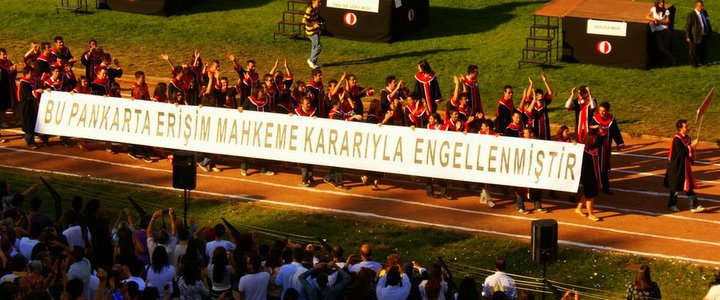
\includegraphics[width=1\textwidth]{project_graphics/banner1.jpg}
  \caption{The banner carried by new grads, 2011}
  \label{fig:Banner_1}
\end{figure}

\textbf{Order slips} (Figure \ref{fig:BankSlips}) are collected from bank office located at Technopolis of Middle East Technical University. They are used to record the order of customers. I realized that back of them are empty and appropriate for writing. Further there many others are waiting on the bin. After this experiment I really convinced that I am really looking for trash everywhere every time. The act of collecting spread through the every moment of life. 

\textbf{A4 photocopy papers} are collected from Bilkent Computer Laboratory. In every lab there is a one printer. However when someone wants to print computers suggest firstly printer on the room 307. This result in many confusions and extra prints. I explored this place during my thesis research. I went there to print out draft of my thesis. I encountered that many papers are leaved on the tables.  The reason of why they are leaved behind is not obvious but technical errors, printing wrong versions and extra copies can be easily guessed after a little observation. Nobody cares others print out. Papers are mostly composed of lecture notes. I collected many papers from there and they are used as a page of notebooks. I do not know owner of them and possibly users of notebooks so. However it will increase our realization of what other students in this university are dealing with.

Similar type of papers are also taken from my friend. They are composed of his lecture notes. He donated them to the project.

Collected items are not limited with these but for the others there are no special memory. Tea bags, collected packages from the streets are some of them.

Most of the materials that I collect are mass produced items. Generally their usage fall into the two category; education and food industry. They are found on public places. They are not personal objects like in the work of Tracey Emin’s \quotes{My Bed} even if it can be claimed that the collected papers from the laboratory contains personal travel tickets. Identity of owner are not certain.

% Elimde bazılarının fotoğrafları (kayıtları) var bazılarının ise yok.

% burdaki dikkate alinan sey satilan bir sey olmadigdi. Kütuphanede ise aslinda bunun bir reklam anlami tasiyip tasimayagi idi. Bilkent labindakiler ise bunukomsenin almayacagi dokunmayacagi yonundeydi. E napalim artik. Insanlarla konustukca farkli seyler dusunuyorum.

% ozellikle resterantlardan bunkari tplarken, genekde garsonlar hemen almaya calisiyorlardi. Ben topladigimi soylerken bu zman yenisini getirmeyi teklif ediyorardi. Bu benim onceden bahsettigimaz tuketme kurali ile celismekteydi ve ben bunu reddediyordum.



%****************************************
\subsection{Transformation}
At one side while paper is being collected, on the other side I started to make experiments with the material. I questioned what else can be made with these collected materials and tried to cover (wrap out) objects and plants in the public. However these do not give the result what I want. People cannot interact with these and possibly they will turn to trash again. For that reason the first approach which is making notebooks are more appropriate to accomplish the purpose.

\begin{figure}
  \begin{subfigure}[b]{0.48\textwidth}
    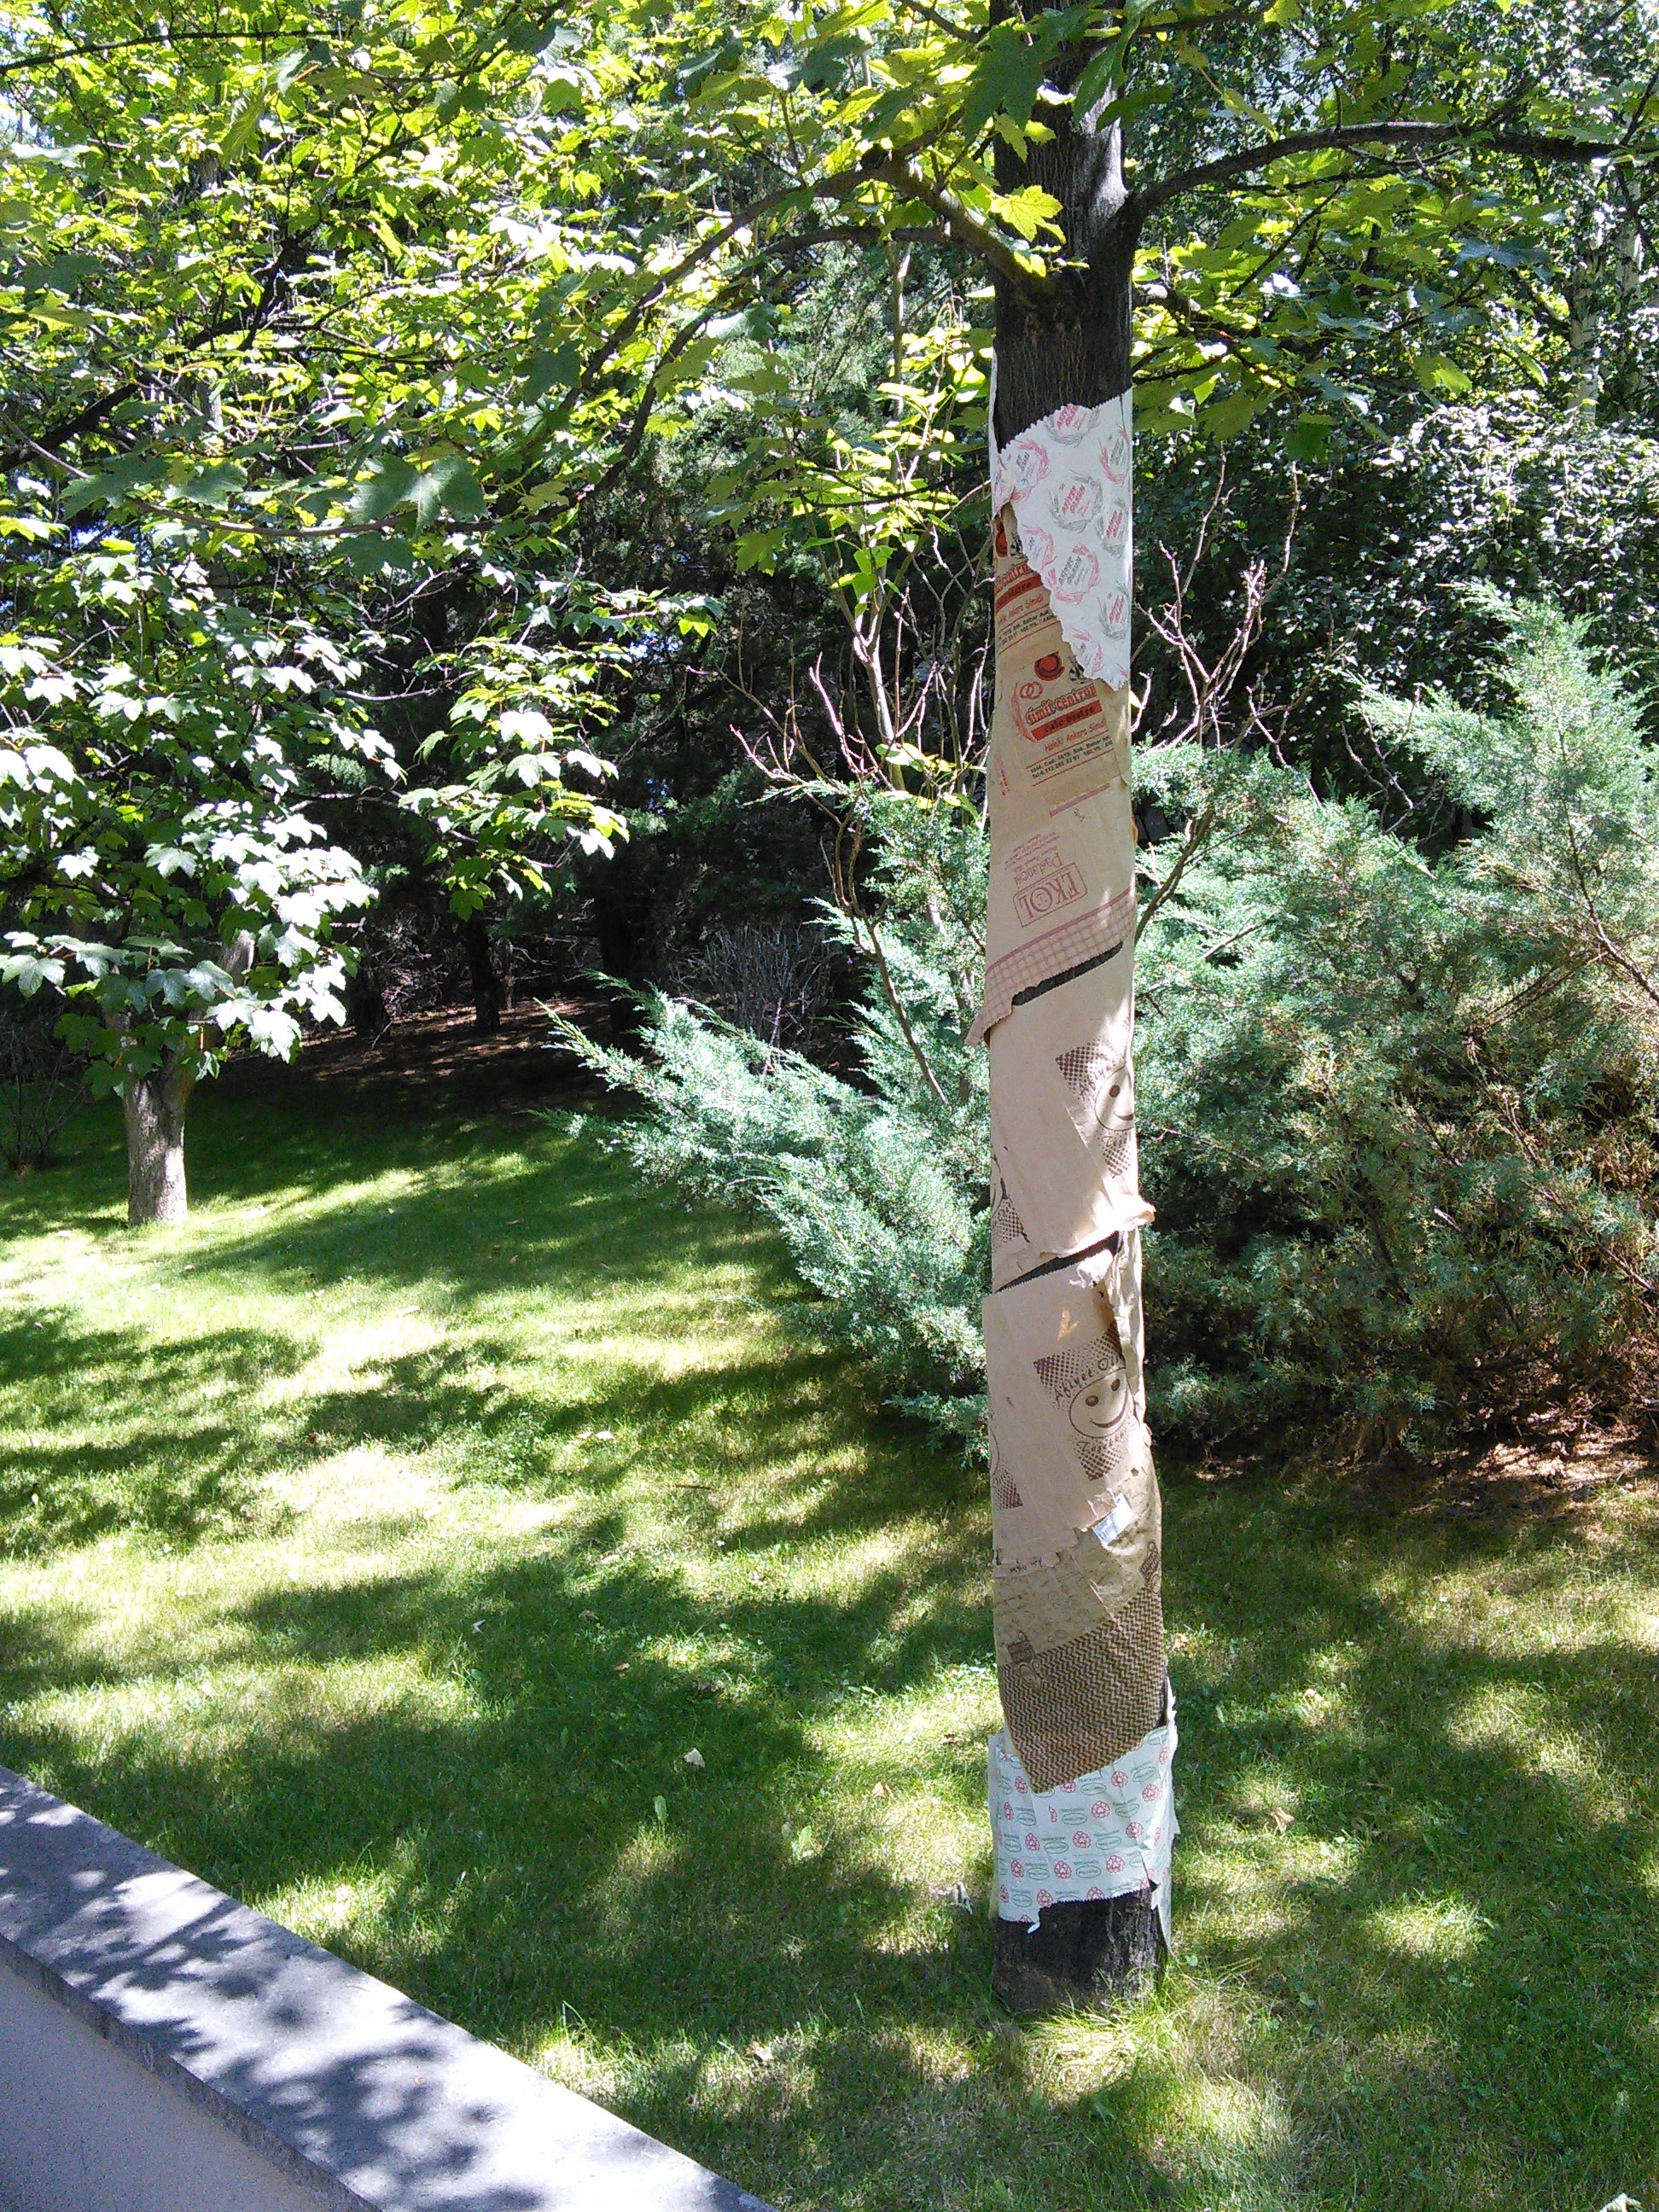
\includegraphics[width=\textwidth]{project_graphics/tree_experiment1.jpg}
  \end{subfigure}
  \hfill
  \begin{subfigure}[b]{0.48\textwidth}
    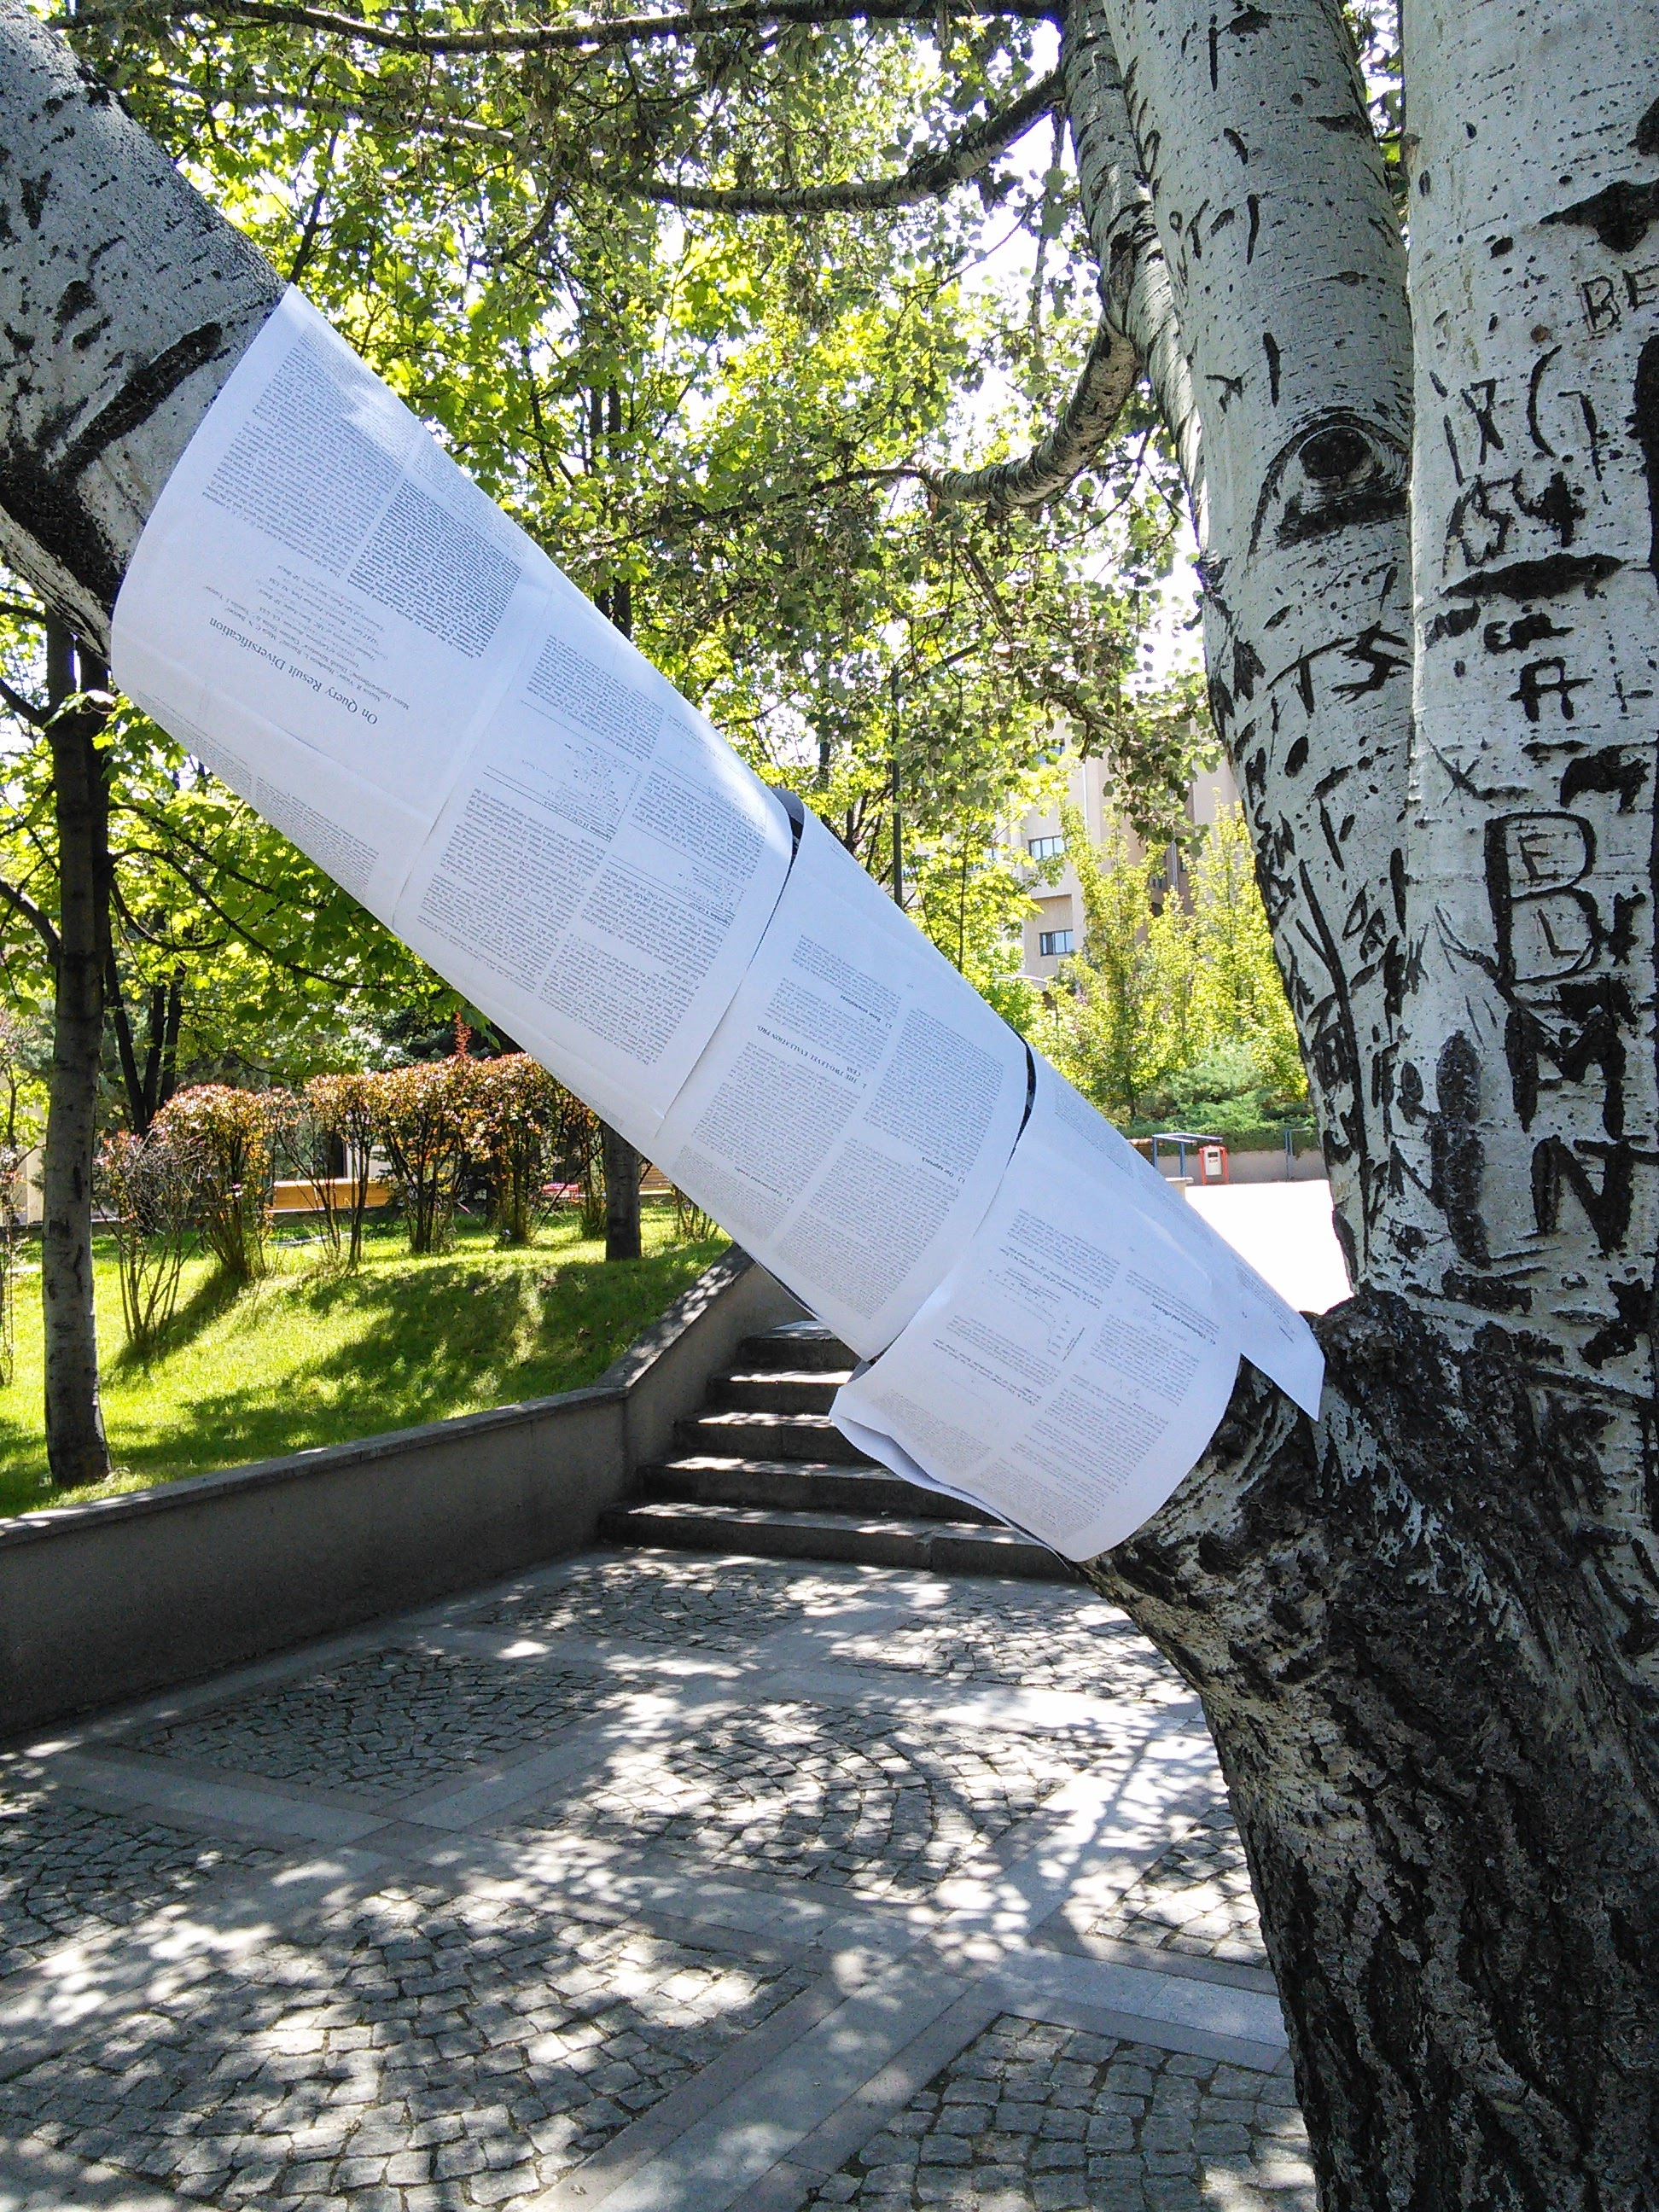
\includegraphics[width=\textwidth]{project_graphics/tree_experiment2.jpg}
  \end{subfigure}
  \caption{Experiments with collected papers}
  \label{fig:ExperimentWithPaper}
\end{figure}

% [notebooks]
There are two main parts of notebooks; cover and pages. Papers that are mostly blank (empty) are used inside of the notebooks for writing. Others that are solid and colorful are used as a cover for notebooks. Mixing (juxtaposing) materials is main method in the production process. I combine different papers and packages. I try to generate every possible combination. The purpose is to create as many alternatives as I can because trash is ignored and people do not give it alternatives. Therefore these notebooks provide many alternatives to show that otherwise is possible. 

Technically papers combined together by sewing and gluing. I learned sewing techniques from my mother and the gluing part is trivial. For this project I need to produce dozens of notebooks. However through time I started to produce them more rapid by improving my technique. One of the struggles that I faced is to punch holes with needle. At this process I cracked a needle. Later I discovered that with the help of pushpin punching the holes becomes more easy. After punching holes I just followed the holes with needle. I used nylon yarn which is solid and thin. Being thin is important it must fit into the opened holes. After sewing them I fixed the yarn with hole by gluing to make it more solid.

I followed the methods of Dada poem to mix the papers used inside of the notebooks. I changed their order and direction. 
\cite{tzara1977seven}, gave the following instructions on how \quotes{[t]o make a Dadaist Poem}:

\begin{quote}
Take a newspaper. Take some scissors. Choose from this paper an article the length you want to make your poem. Cut out the article. Next carefully cut out each of the words that make up this article and put them all in a bag. Shake gently. Next take out each cutting one after the other. Copy conscientiously in the order in which they left the bag. The poem will resemble you. And there you are ---an infinitely original author of charming sensibility, even though unappreciated by the vulgar herd.
\end{quote}

Size of the paper used inside of the notebooks are mostly equal to the size of an A4 sheet (dimensions: 210mm x 297mm). There are different dimensions of notebooks. Most of them are half of A4 sheet or quarter of it. Collected papers' dimension shape the size of the notebooks. Usage of papers differs among the notebooks. Especially for the papers taken from Varuna Gezgin written part is folded inward by hiding it. However for the ones collected from Bilkent Computer Laboratory written side of it is left open. Their content comes from various students whose departments are also various. In other words, they offer great diversity and they are mixed to allow different interpretations. Further they provide what students from other departments work on.

% TODO defterin yakından fotoğrafları

% TODO defter dikme yönteminin fotoğrafı

The tools used in the making of notebooks are as follows; needle, sewing thread, scissors, utility knife, pushpin, silicone, caulking guns.

While transforming collected materials my method can be explained with the term upcycling mentioned at the end of the chapter 1. Further I tried to use objects already at hand. In other words I followed the \textit{bricolage} technique. However I have to do buy some tools for my work. Therefore it is hard to consider it as \textit{bricolage} but my intention is to follow it.

Moreover I have reviewed other notebook projects. Notable ones are \textit{The Sketchbook Project} and \textit{myDetour} from Moleskine. In these projects anyone who bought the notebooks from them can participate and send their notebooks filled with illustrations and paintings. These projects can be seen as crowd-sourced library. Further the pages of the notebooks are available at online. After checking sketches in these notebooks, the diversity of them surprised me a lot. It forced me think that the transformation process is not limited with the production of notebooks from trash. After notebooks are given to the people, their transformation will continue. Therefore I think the process of transformation is a continuous act.

% The purpose is here to increase the diversity.

% Çok basit bir şekilde çöp olarak görülen bir şeyi başka bir şey olarak görmek keyifli bir şey benim için. zaten dönüştürmek kullanmak için topluyorum.

% Dönüştürme sebepleri. Neden sadece toplamakla yetinmiyorum. Yeni kompozisyonlar oluşturmak istiyorum. Farklı karşımlar elde etmek istiyorum. Bir tür şaşırtmak durumu... Beklenmeyeni yapmak... En olmadık malzeme çöple çalışmak bu yüzden önemli benim için.

% [Artistic tactics] Here I followed some tactics to accomplish my purposes. Easy to carry while traveling. Small notebooks. Placing them to their routes.

% bi de ben bunu insanlara vermek istiyordum o yüzden defter iyi bir şey. ve bu benim aslında bir taktiğim arkadaş. defter insanın yanında taşıdığı kullandığı bir şey. sadece galeri de olmayan başka alanlara da sızan bir şey olması önemli. 



%****************************************
\subsection{Demonstration}
After producing notebooks the most important point is to present and reach to people. Main question is how to give them to people. Starting point is to stack the notebooks onto the each other, and there are other ideas like putting them inside a waste bin to re-do the action of throwing away. Afterwards somehow they should understand that these notebooks can be taken. I set up models and tried some installations of them.

\begin{figure}
  \begin{subfigure}[b]{0.31\textwidth}
    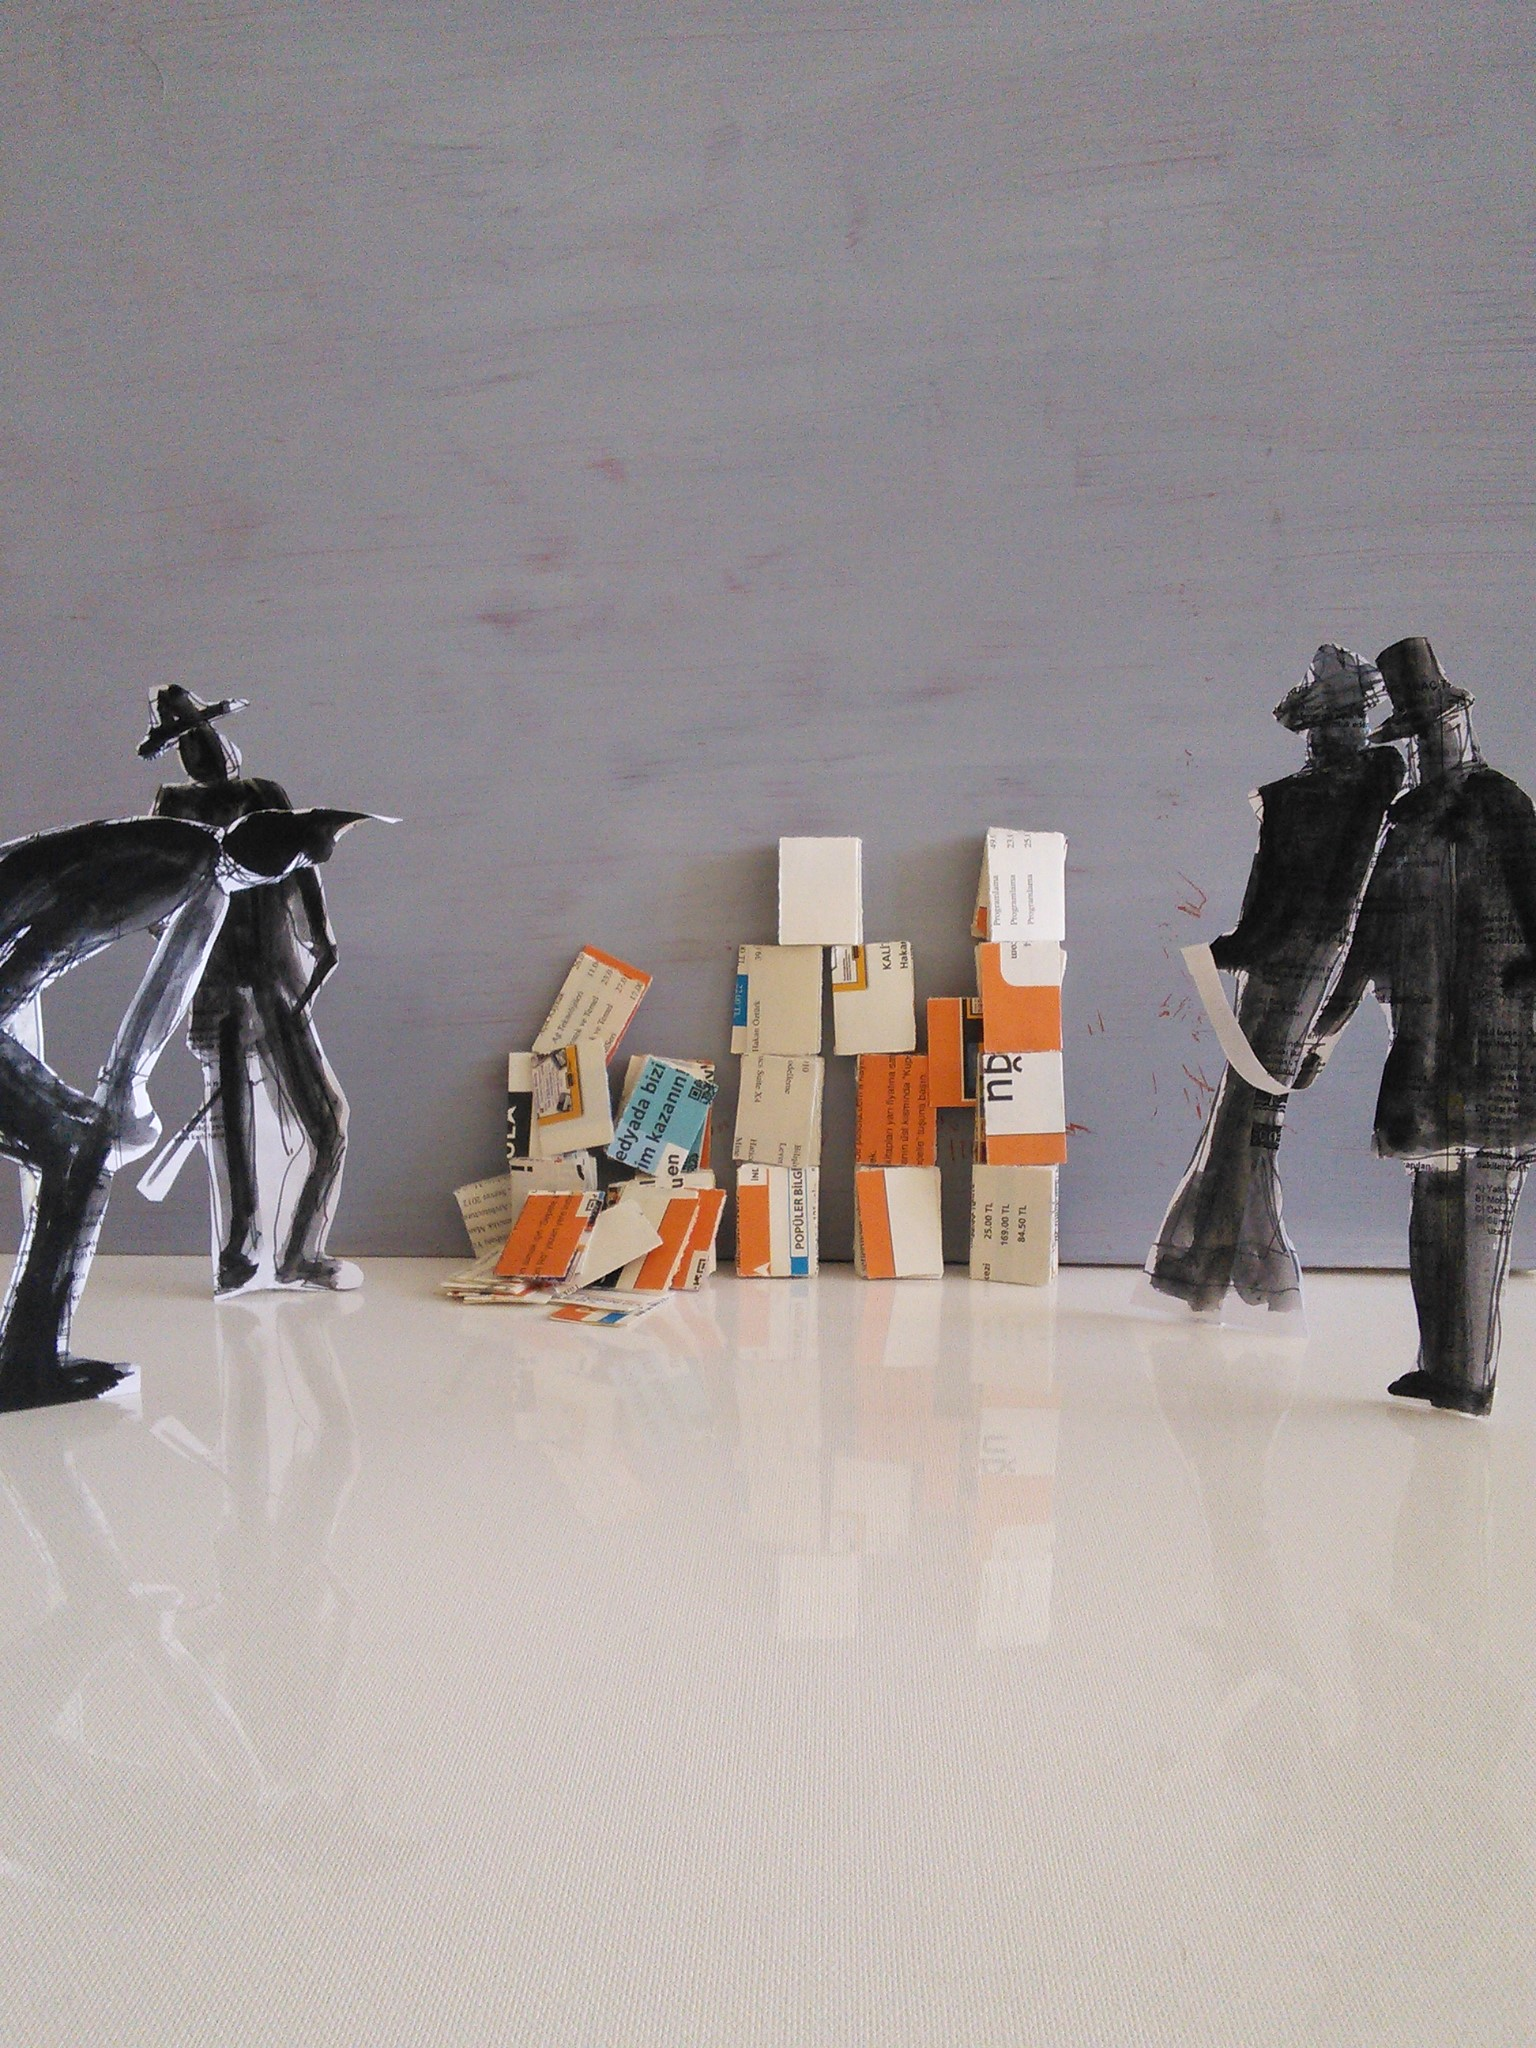
\includegraphics[width=\textwidth]{project_graphics/exhibition1.jpg}
    \label{fig:exhibition1}
  \end{subfigure}
  \hfill
  \begin{subfigure}[b]{0.31\textwidth}
    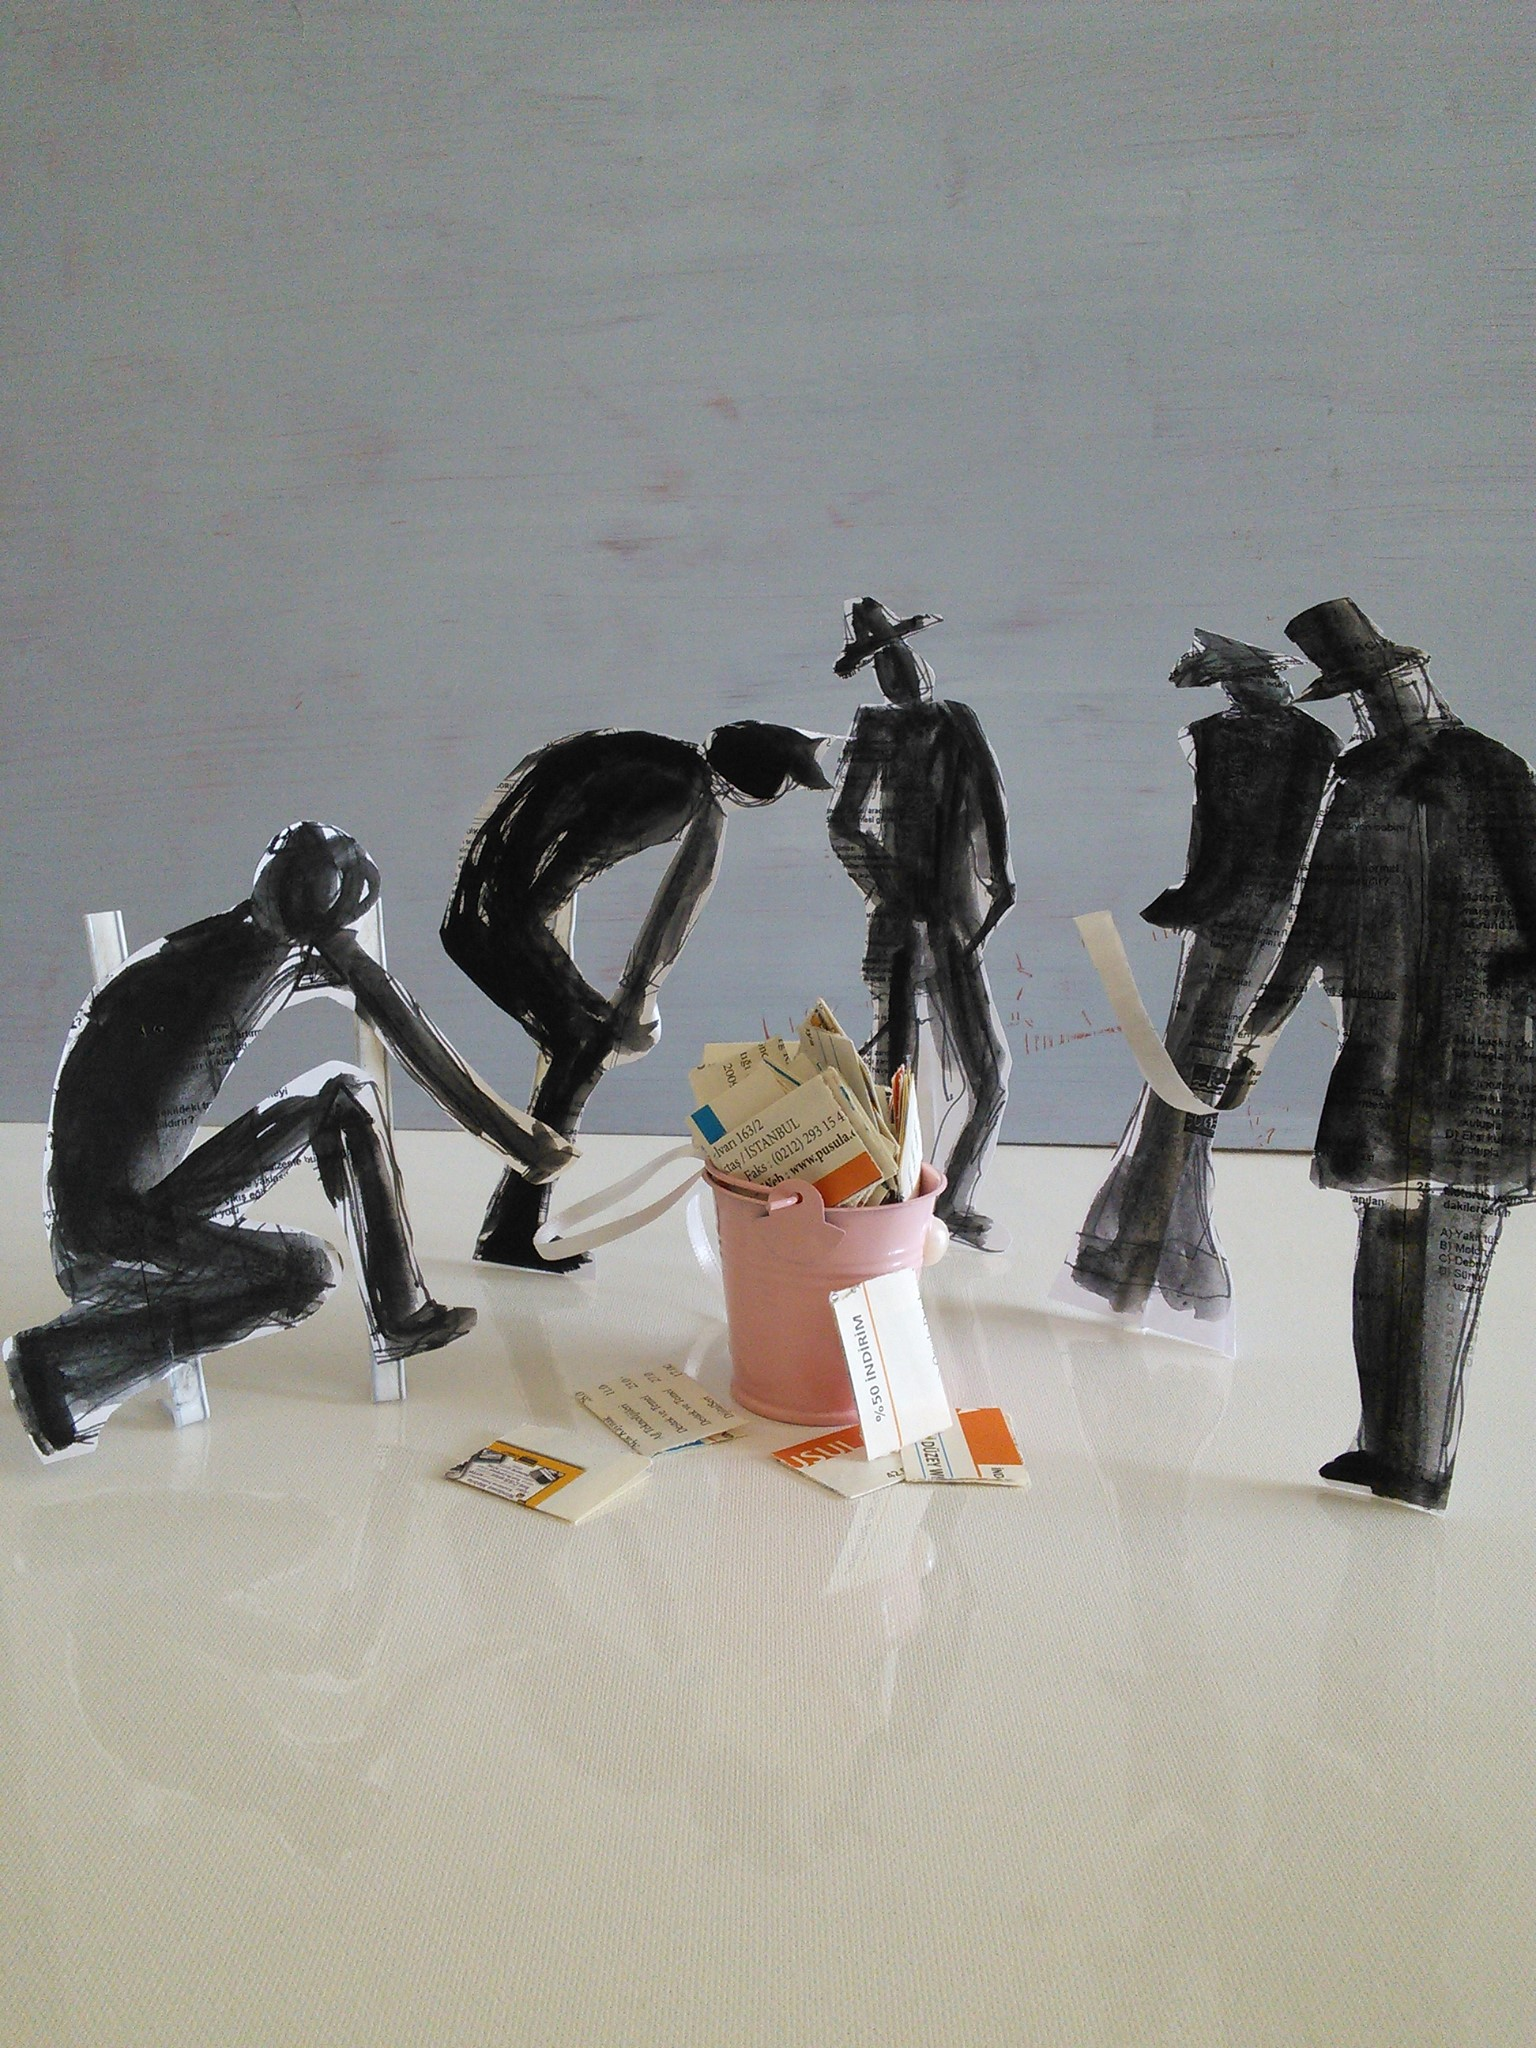
\includegraphics[width=\textwidth]{project_graphics/exhibition2.jpg}
    \label{fig:exhibition2}
  \end{subfigure}
  \hfill
  \begin{subfigure}[b]{0.31\textwidth}
    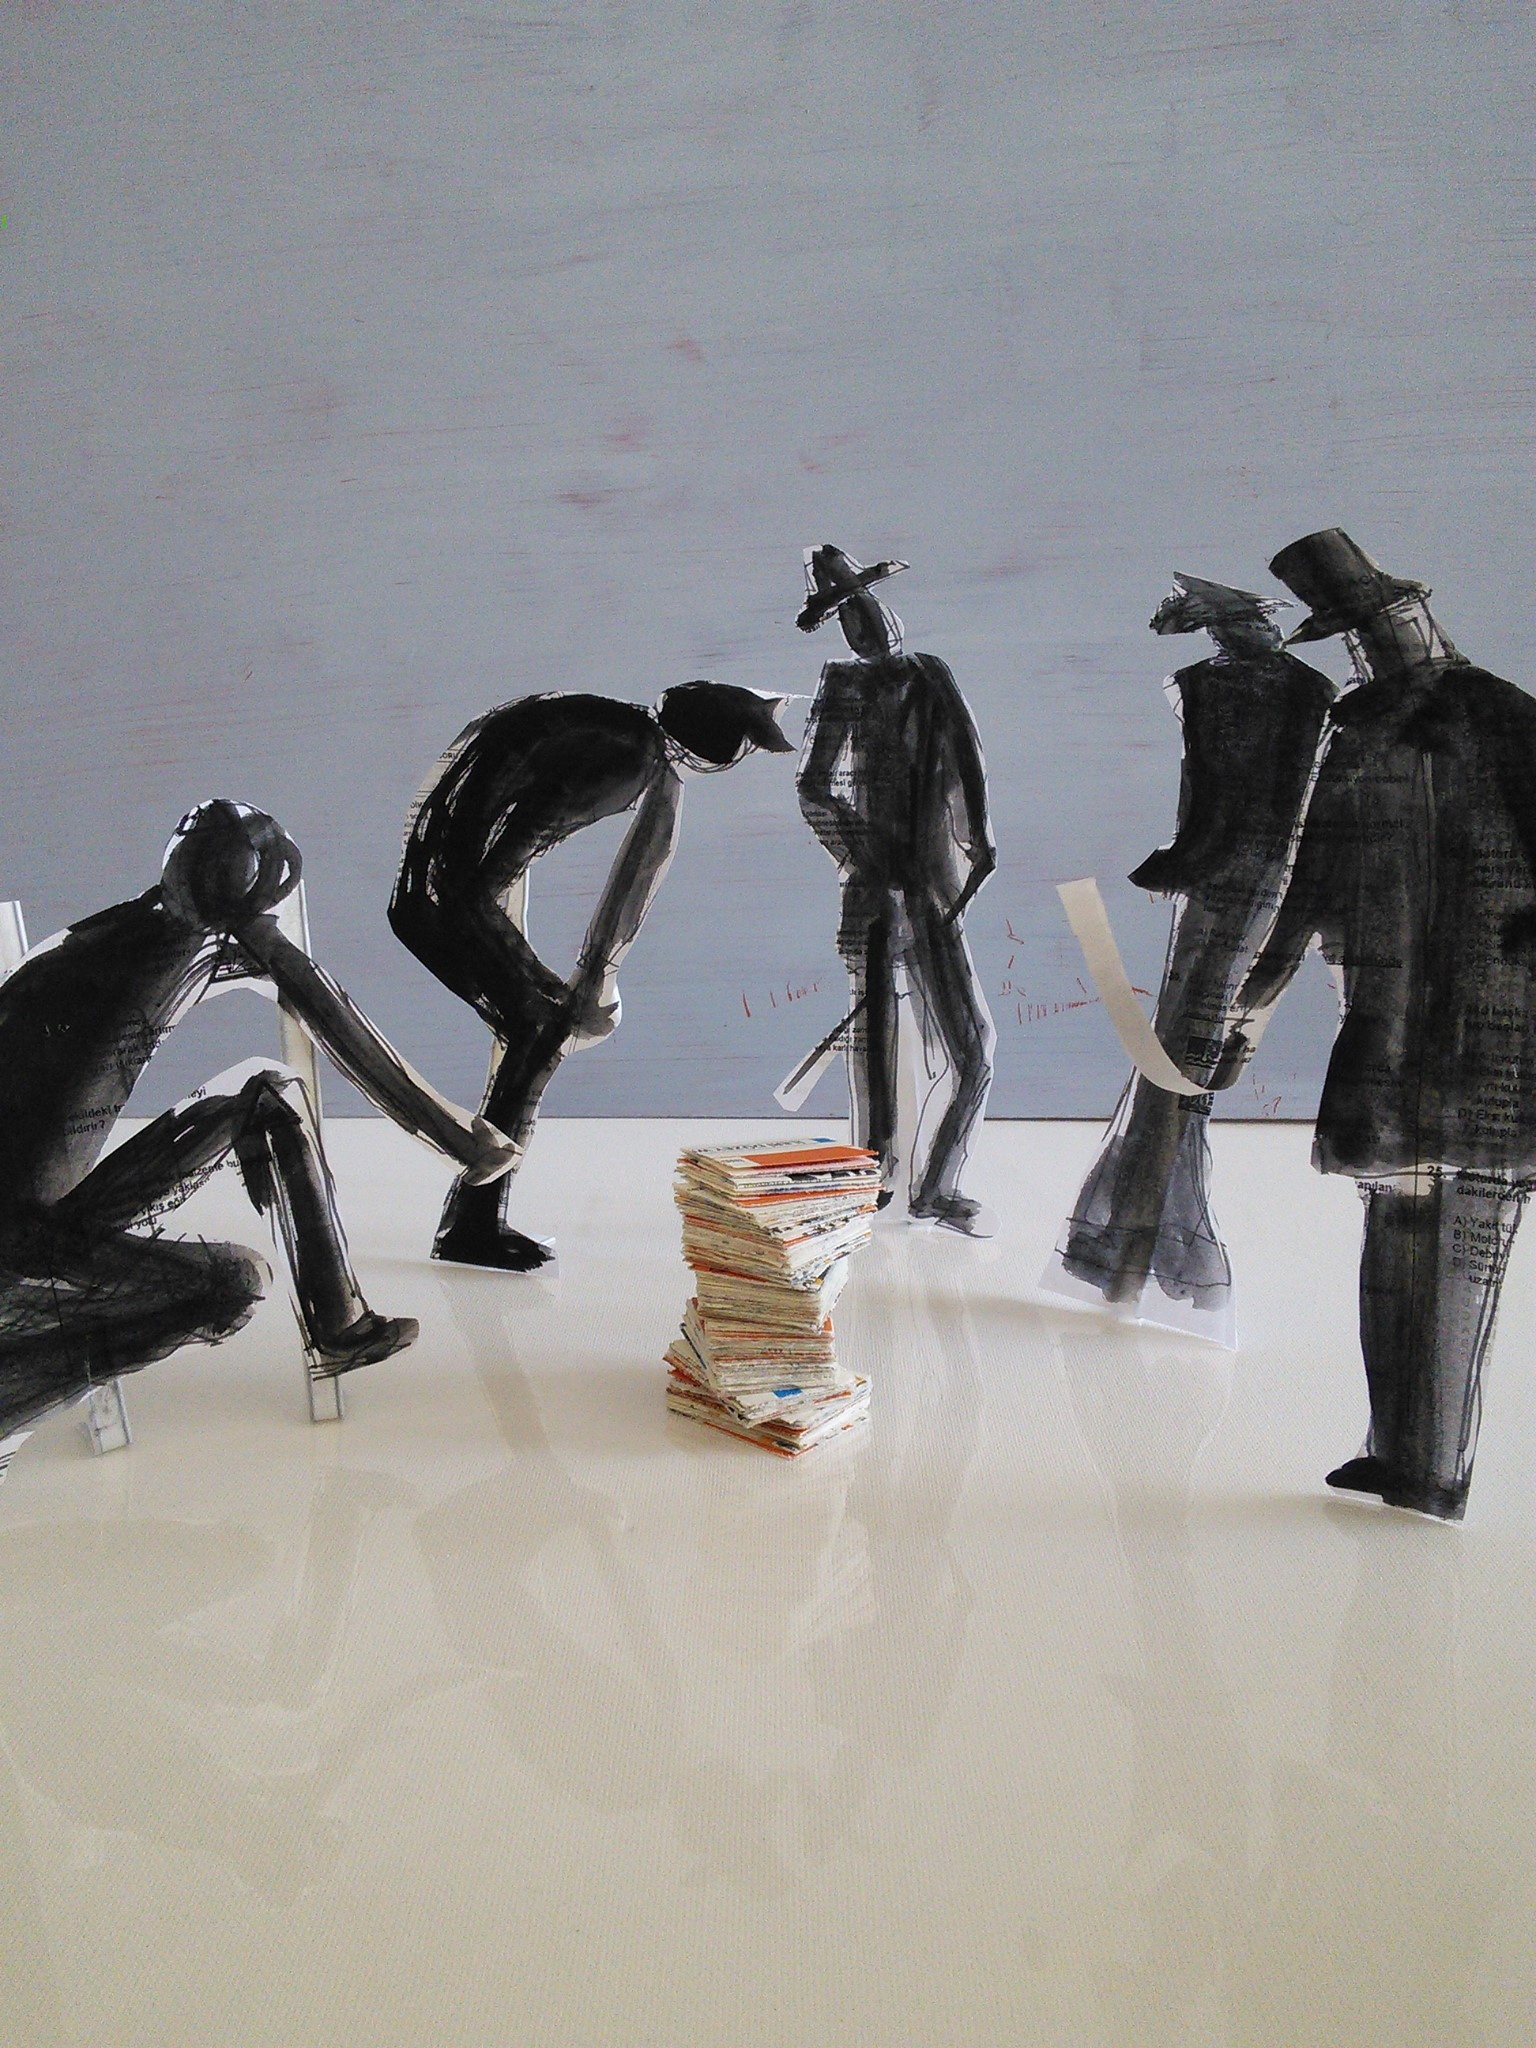
\includegraphics[width=\textwidth]{project_graphics/exhibition3.jpg}
    \label{fig:exhibition3}
  \end{subfigure}
  \caption{Installation experiments with models}
  \label{fig:exhibition}
\end{figure}

They were early interpretations and ideas. I imagined an exhibition environment to place notebooks (Figure \ref{fig:exhibition}). Different placements were tried. All of them looked like a sculpture. I have inserted no special meaning as sculpture to this objects. I also afraid that people will not interact with them and look them away. My purpose is give people. Aim is to spread the idea by making something useful from trash and to increase diversity, to encourage people in order to embrace the trash.

These experiments showed me that I need to place them to the locations where people frequently visit. It must be inside of the life. As it is collected publicly it must be showed publicly. Thus the project can reach more audience. It will spread and can be showed in different contexts. Notebooks can move with people.

To hold notebooks together I made several small boxes from discarded card boxes. Notebooks were put inside of them. In the production phase of the boxes, I discovered that my folded notebooks are fit into the many card boxes. In other words dimensions of them are not very different. This property of items make my production more easier. It shows that industrial system supports the reuse of the object with less effort in this way.

% TODO Rubbish Theory showing off.

% TODO [Why giving away?] Felix Gonzales Torres, Unlimited Editions.

% The \quotes{Untitled} series of Felix Gonzales Torres inspired me a lot when deciding giving notebooks away. He has created variations on the theme of the “stack,” which consists of “unlimited” editions of offset prints. Visitors can take a copy of them. 

% TODO insanlar bu defterleri neden alsınlar.

% [Website]

% websitesinde amac bunlari anlatabilmekti. 
% Anlattığım bir çok şeyi sadece deftere bakarak anlamak mümkün değil ve ben bunların insanlara ulaşmasını istiyorum. buradaki seçeneklerden bir tanesi site ile onlara ulaşmaktı. temel sebeplerden bir tanesi bu mediumda ben tecrübeliydim. for the smaller parts what is written on them can not easily understandable. To realize what is the message is you have to bring together all of them again. But It is not possible, therefore website is a very good solution for them.

Beyond all of these for the audience the story of the collected materials is a mystery. Audience are not aware from all of these written in this thesis. I want to reveal the act behind these notebooks. However there is a lot information that can not be fit into the pages of notebooks. For that reason such problems can be clearly solved through a website that store the records of notebooks and collected materials. People can visit the website anytime. Further I am comfortably and confidently fluent in coding and web development. Therefore it is more appropriate for the scope of this thesis.

Notebooks will be given away. They will continue to flow between people. There is a possibility that notebooks can be trashed again. However vice verse is possible. In other words they might turn to durable objects as mentioned in Rubbish Theory. At this time, decision belongs to people. However website serve great functionality here. While the notebooks have potentials to be rubbish, records of them in the website are preserved.



%****************************************
\section{Parts of the Final Work}
As also can be understood by the previous section the project introduced in this thesis have different parts. Each part support the other. They are connected with each other. Different parts lead different inquiries.



%****************************************
\subsection{Notebooks}
Notebooks have been used for different purposes such as drawing, writing and recording, ideas or memorandum by many artists, scientists, and thinkers through the ages. Further the same exists for me and people around me. Although there are digital alternatives of it paper maintains its place in the community.

Through this project handmade notebooks are produced from discarded paper. They are impure, imperfect and different than usual industrial notebooks. They still carry the traces of previous usage. Every one of them have different stories. Combination of various pieces offer new interpretations of writing.

There are different types of notebooks regarding their color, shape, size and combination. They are simple, imperfect and different than usual industrial notebooks, but more importantly they are from trash. Every one of them has a unique serial and with that serial the (hi)story of it can be viewed.

% Meaning of stories behind the process
There are different stories behind the objects. I try to record their stories (by photography and taking notes) but some of them were not possible. However I still use them in the work because even if I missed their story, with their materiality their history reveal themselves. They still have histories but they need to be rewritten. Maybe forgetting all the history maybe creates different notebooks.

Every notebook has unique serial and with this it can be tracked down when it was produced and which materials are used production of it. Serial is generated through the first letter of composed material. 

Giving name is another hard topic for me. However point out the story behind the notebooks and properties of it. These names gives clues about how they are combined what they represent, defines the aspects of them. Name of the paper can be related with this place and related with the meaning. These names captures the memory of notebooks. However for one series I borrowed the idea of nonsense word generation from the Kurt Schwitters. Similar to the the production of the nonsense word \textit{Merz} I decided to name some of the notebooks a nonsense word. There are notebook series that have a name. Here are the name of notebooks and their story:

\textbf{Puzzle.} Papers inside of these notebooks are cut out from very big and long banner (see figure \ref{fig:Banner_1}). Every piece is a part of bigger banner. Pages of paper is similar to the pieces of puzzle. All of them are composes the banner. However they are cut out and give away combining them is not possible but the image of the original one can be viewed on the website.

It provides unique layout for writing and I strongly think that all the notebooks after used have strong visual impact.

As mentioned previously the objects are bring their history. They are not blank, they are heterogeneous and hybrid. It can be one of the examples of this argument. 

\textbf{Reunion.} These notebook’s pages are collected from restaurant Varuna Gezgin, in Ankara. We went there to meet some friends after long time. One of them was coming from Australia, the other one was coming from Norway. They were my friends from the university. We united again at this restaurant. The place has also similar story. Their founders and workers travel around the world. It is a popular restaurant of travelers. The decoration of that place contains a lot of items collected from different sides of the world. The concept of the place and our meeting perfectly matched. Same exist for the papers actually, they are separated from big paper rolls in the factory and by the action making notebooks they are also reunited again. These notebooks represent my memory about the place.

\textbf{Secondhand.} It can be thought that these notebooks are second hand objects. Used by someone else and still appropriate for reusing. Here I wish that these papers and notebooks are used more than twice.

\textbf{Daro.} For some of the notebooks it is not obvious to name them. At this point approach of Kurt Schwitters provides me a way. He generated his frequently used word \textit{Merz} from an advertisement. It is a nonsense word and used in most of his works. I followed what he did and generated a word from the papers that used inside of the notebooks. I use the word \textit{Daro} extracted from \textit{Vardaroma Dondurmacısı} for the ones whose story are not obvious and significant. The word found one the of papers collected from near the printer inside of computer laboratory.



%****************************************
\subsection{Exhibition}
Especially exhibition of notebooks is the most hard topic in the development of project. To find an appropriate place for the notebooks is a great challenge for me. Main idea is here to find a place that can also be considered as an alternative art space because in every dimension alternative is seek through the project. It must not only fit inside of white cube and must reach to audience. Therefore frequently visited places is a perfect locations for the project.

Bilkent library and computer laboratory are one of the places where notebooks are placed inside of boxes made from card boards (Figure \ref{fig:BilkentLibrary}-\ref{fig:BilkentLaboratory}).  Libraries are places where books are reused and shared among many people. It can be viewed as a place of sharing culture. Further it is a place that students from several department visit the same location. Particularly in Bilkent there are small papers to write down the shelve numbers of books. It is a great place to leave notebooks there because people already need something to write. They can find notebooks when they need them. For the computer laboratory case, the main purpose is to provide an alternative near the place where mostly papers are carelessly wasted.

\begin{figure}[!tbp]
  \begin{minipage}[b]{0.48\textwidth}
    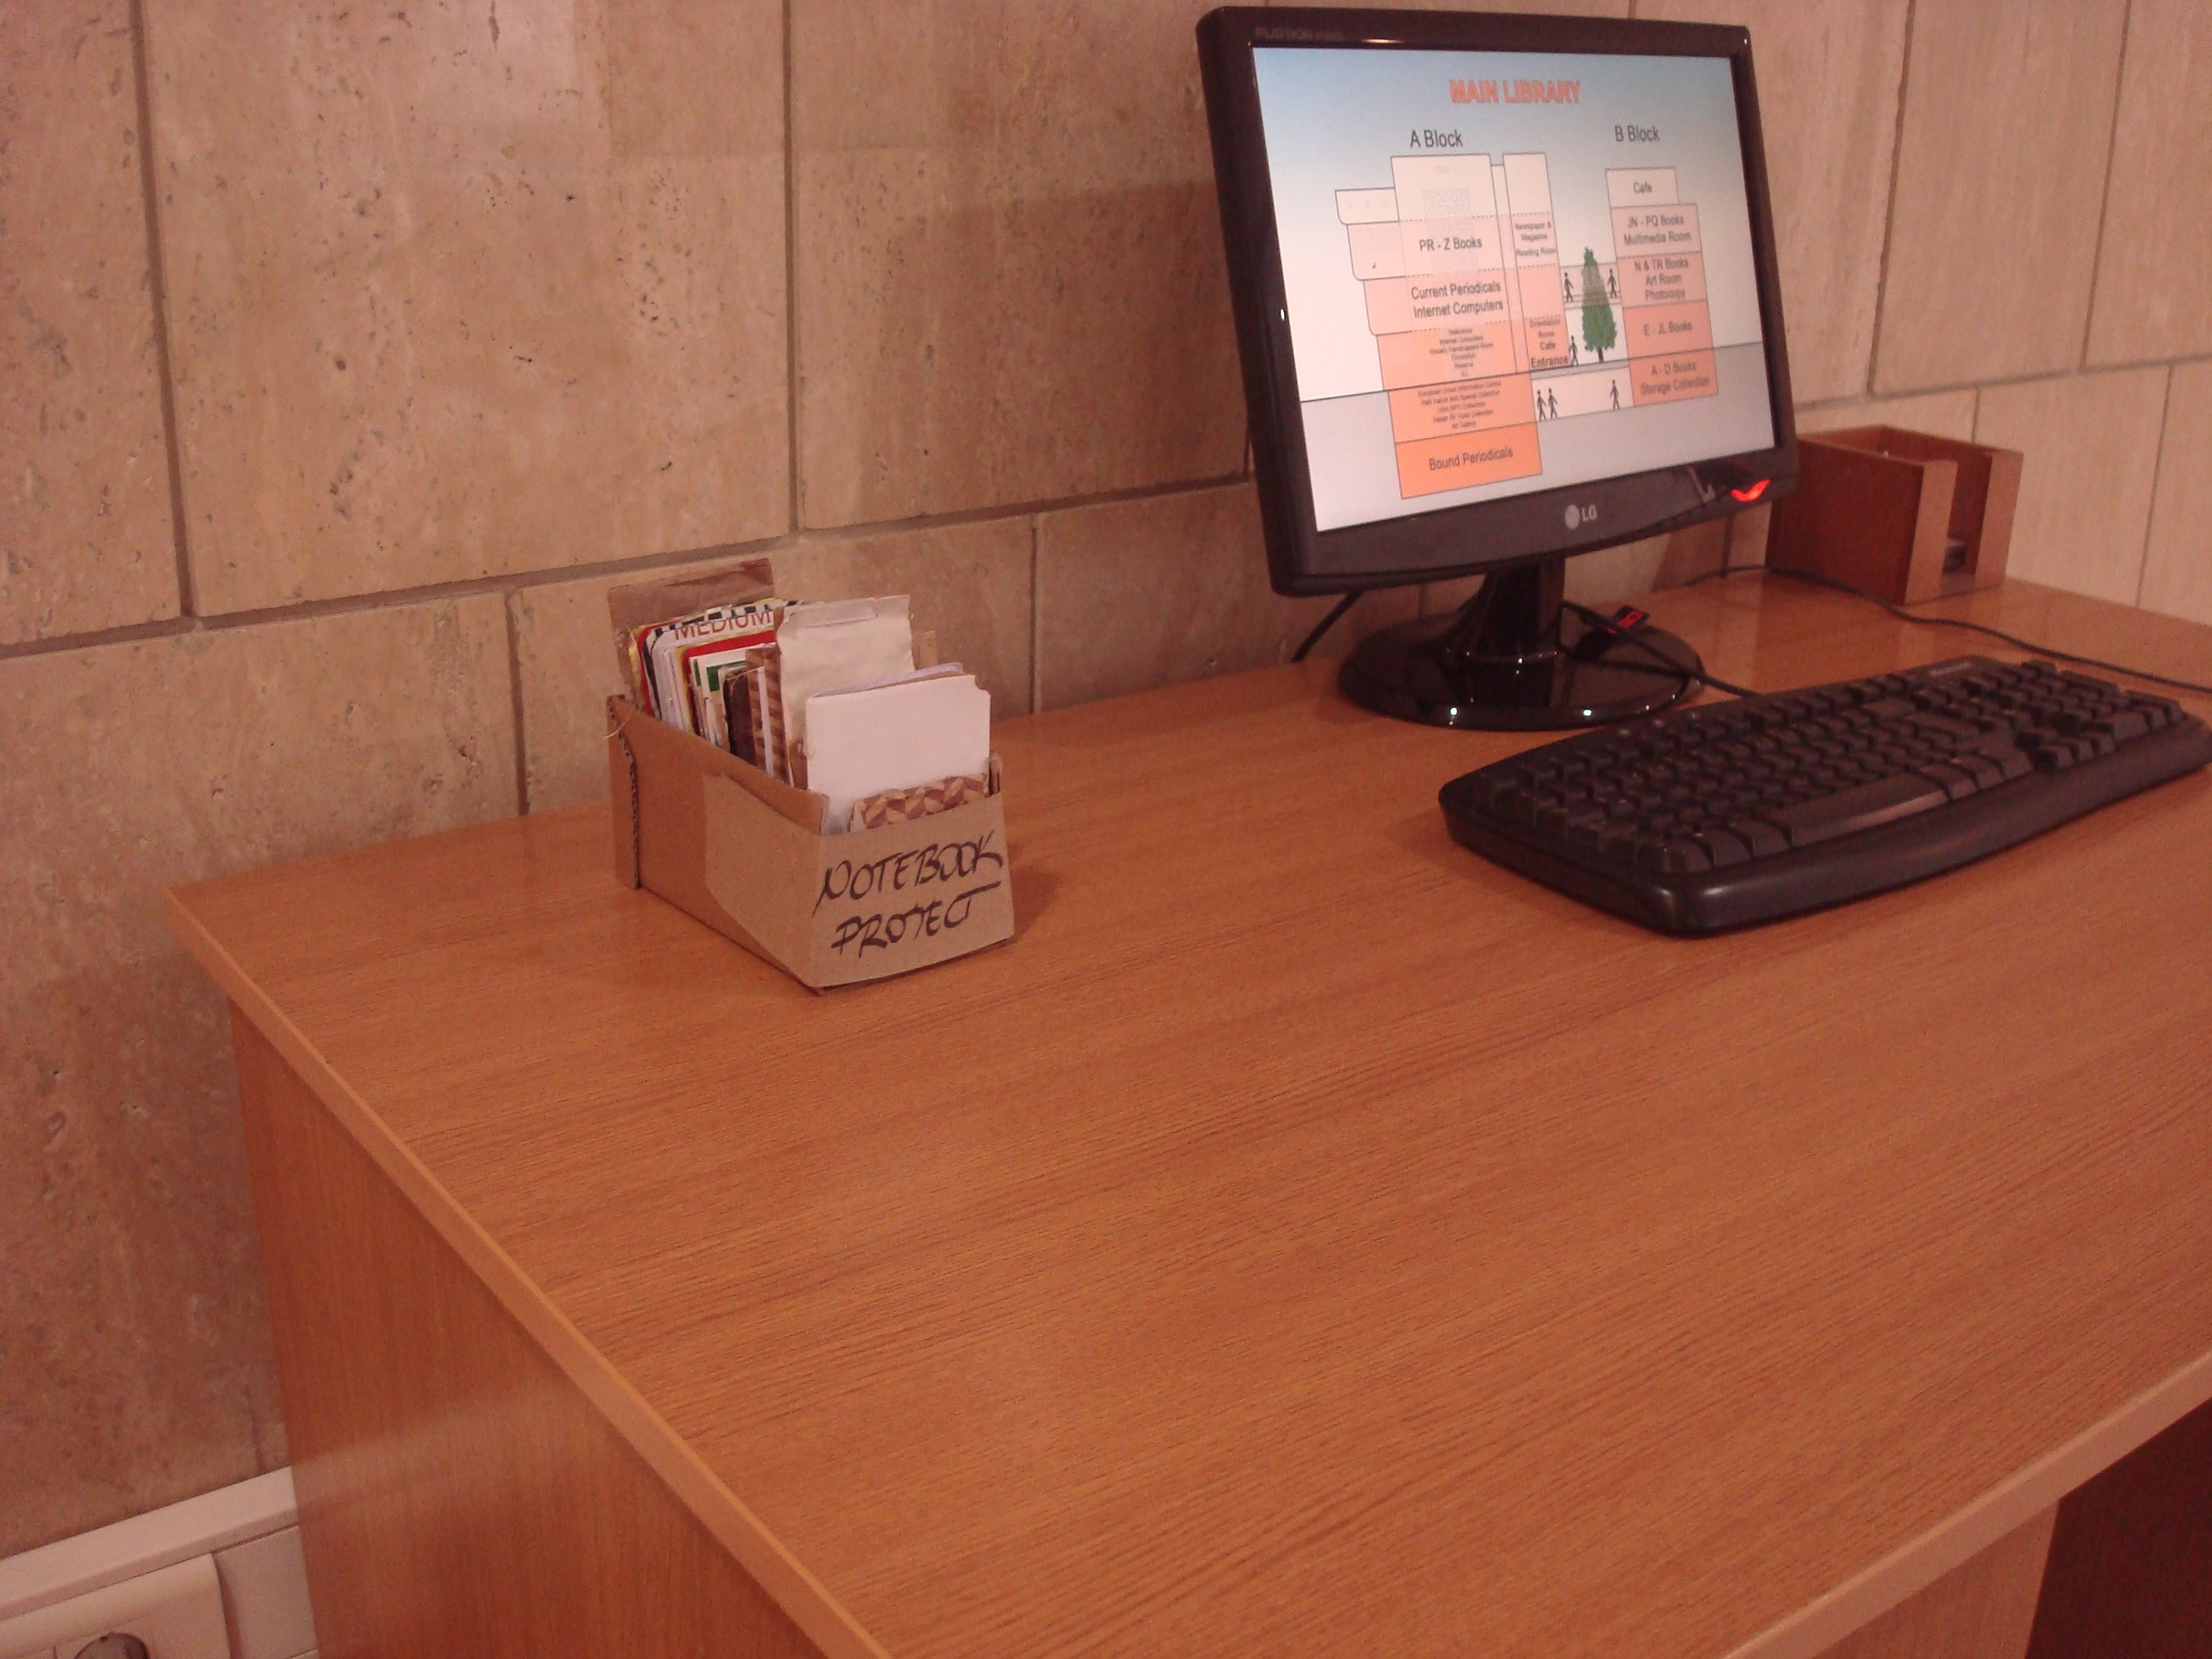
\includegraphics[width=\textwidth]{project_graphics/bilkent1.jpg}
    \caption{Sample placement at Bilkent Library}
    \label{fig:BilkentLibrary}
  \end{minipage}
  \hfill
  \begin{minipage}[b]{0.48\textwidth}
    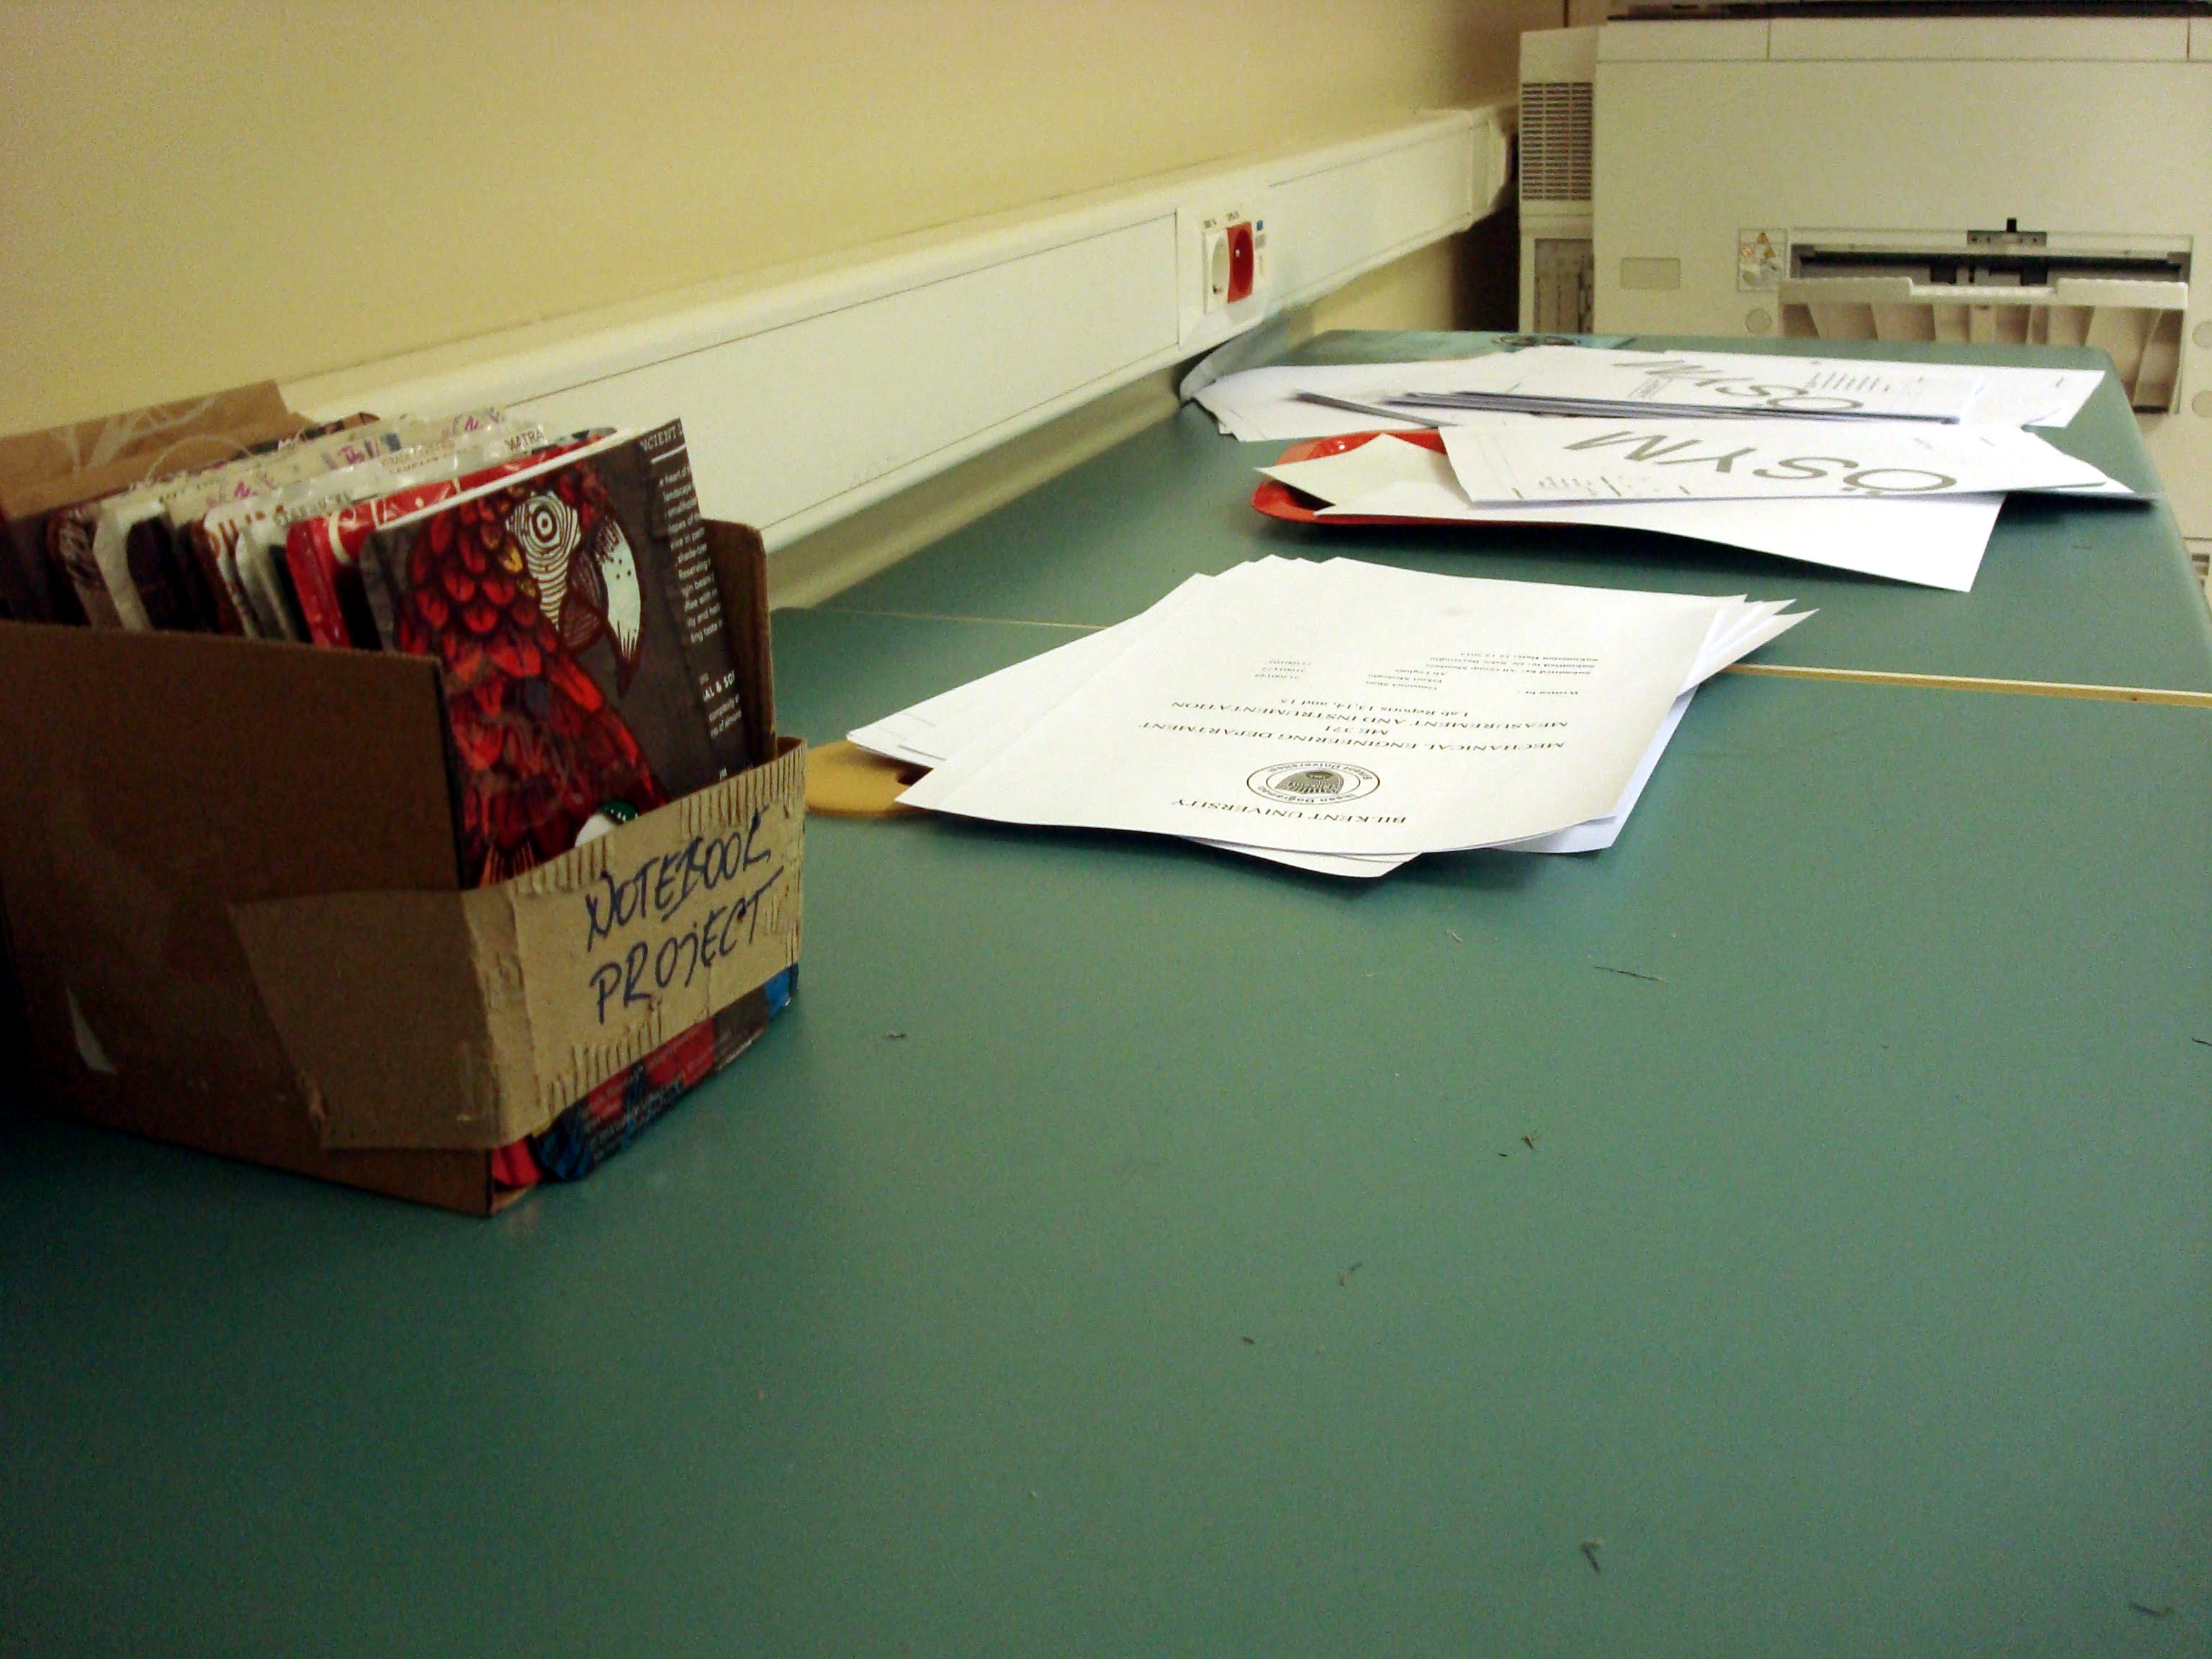
\includegraphics[width=\textwidth]{project_graphics/bilkent2.jpg}
    \caption{Sample placement at Bilkent Computer Laboratory}
    \label{fig:BilkentLaboratory}
  \end{minipage}
\end{figure}

% bir çok insanın ortaklaşa kullandığı bir alan. kesişim alanı. bir tanesi de özellikle zaten toplanan yer. insanların defterlerle karşılaşmalarını istiyorum.

% Torun
Through this project another exhibition alternative is thought. In the notable museums and art galleries there are gift shops that people can buy souvenirs. Often they are mass produced imitations and replicas of well-known artists work embedded various objects such as cover on the notebooks. At this point I image an art space you can get these types of items freely. In other words alternative to the existing approach this types of gadgets. Another alternative interpretation can be giving away different that the industrial items such as notebooks from trash as in my project. For this type of approach Torun is a great place to show my notebooks and give them away. Torun describes itself as a place for free place for sharing art. The place is open to everybody and makes open call to any artist. There are no security cameras on this gallery therefore no one is watching you at there. The project is shared with Torun and it is accepted. 

I used wooden market boxes to lift up them from ground to more reachable height. It is hole body of stand to put notebooks. Notebooks are placed on the top box and below them I just put the collected items to provide for those who want to make their own notebook. People can get them both. Further it reveals the process of the production of the notebooks and shows the previous state of the materials.

\begin{figure}
  \begin{subfigure}[b]{0.48\textwidth}
    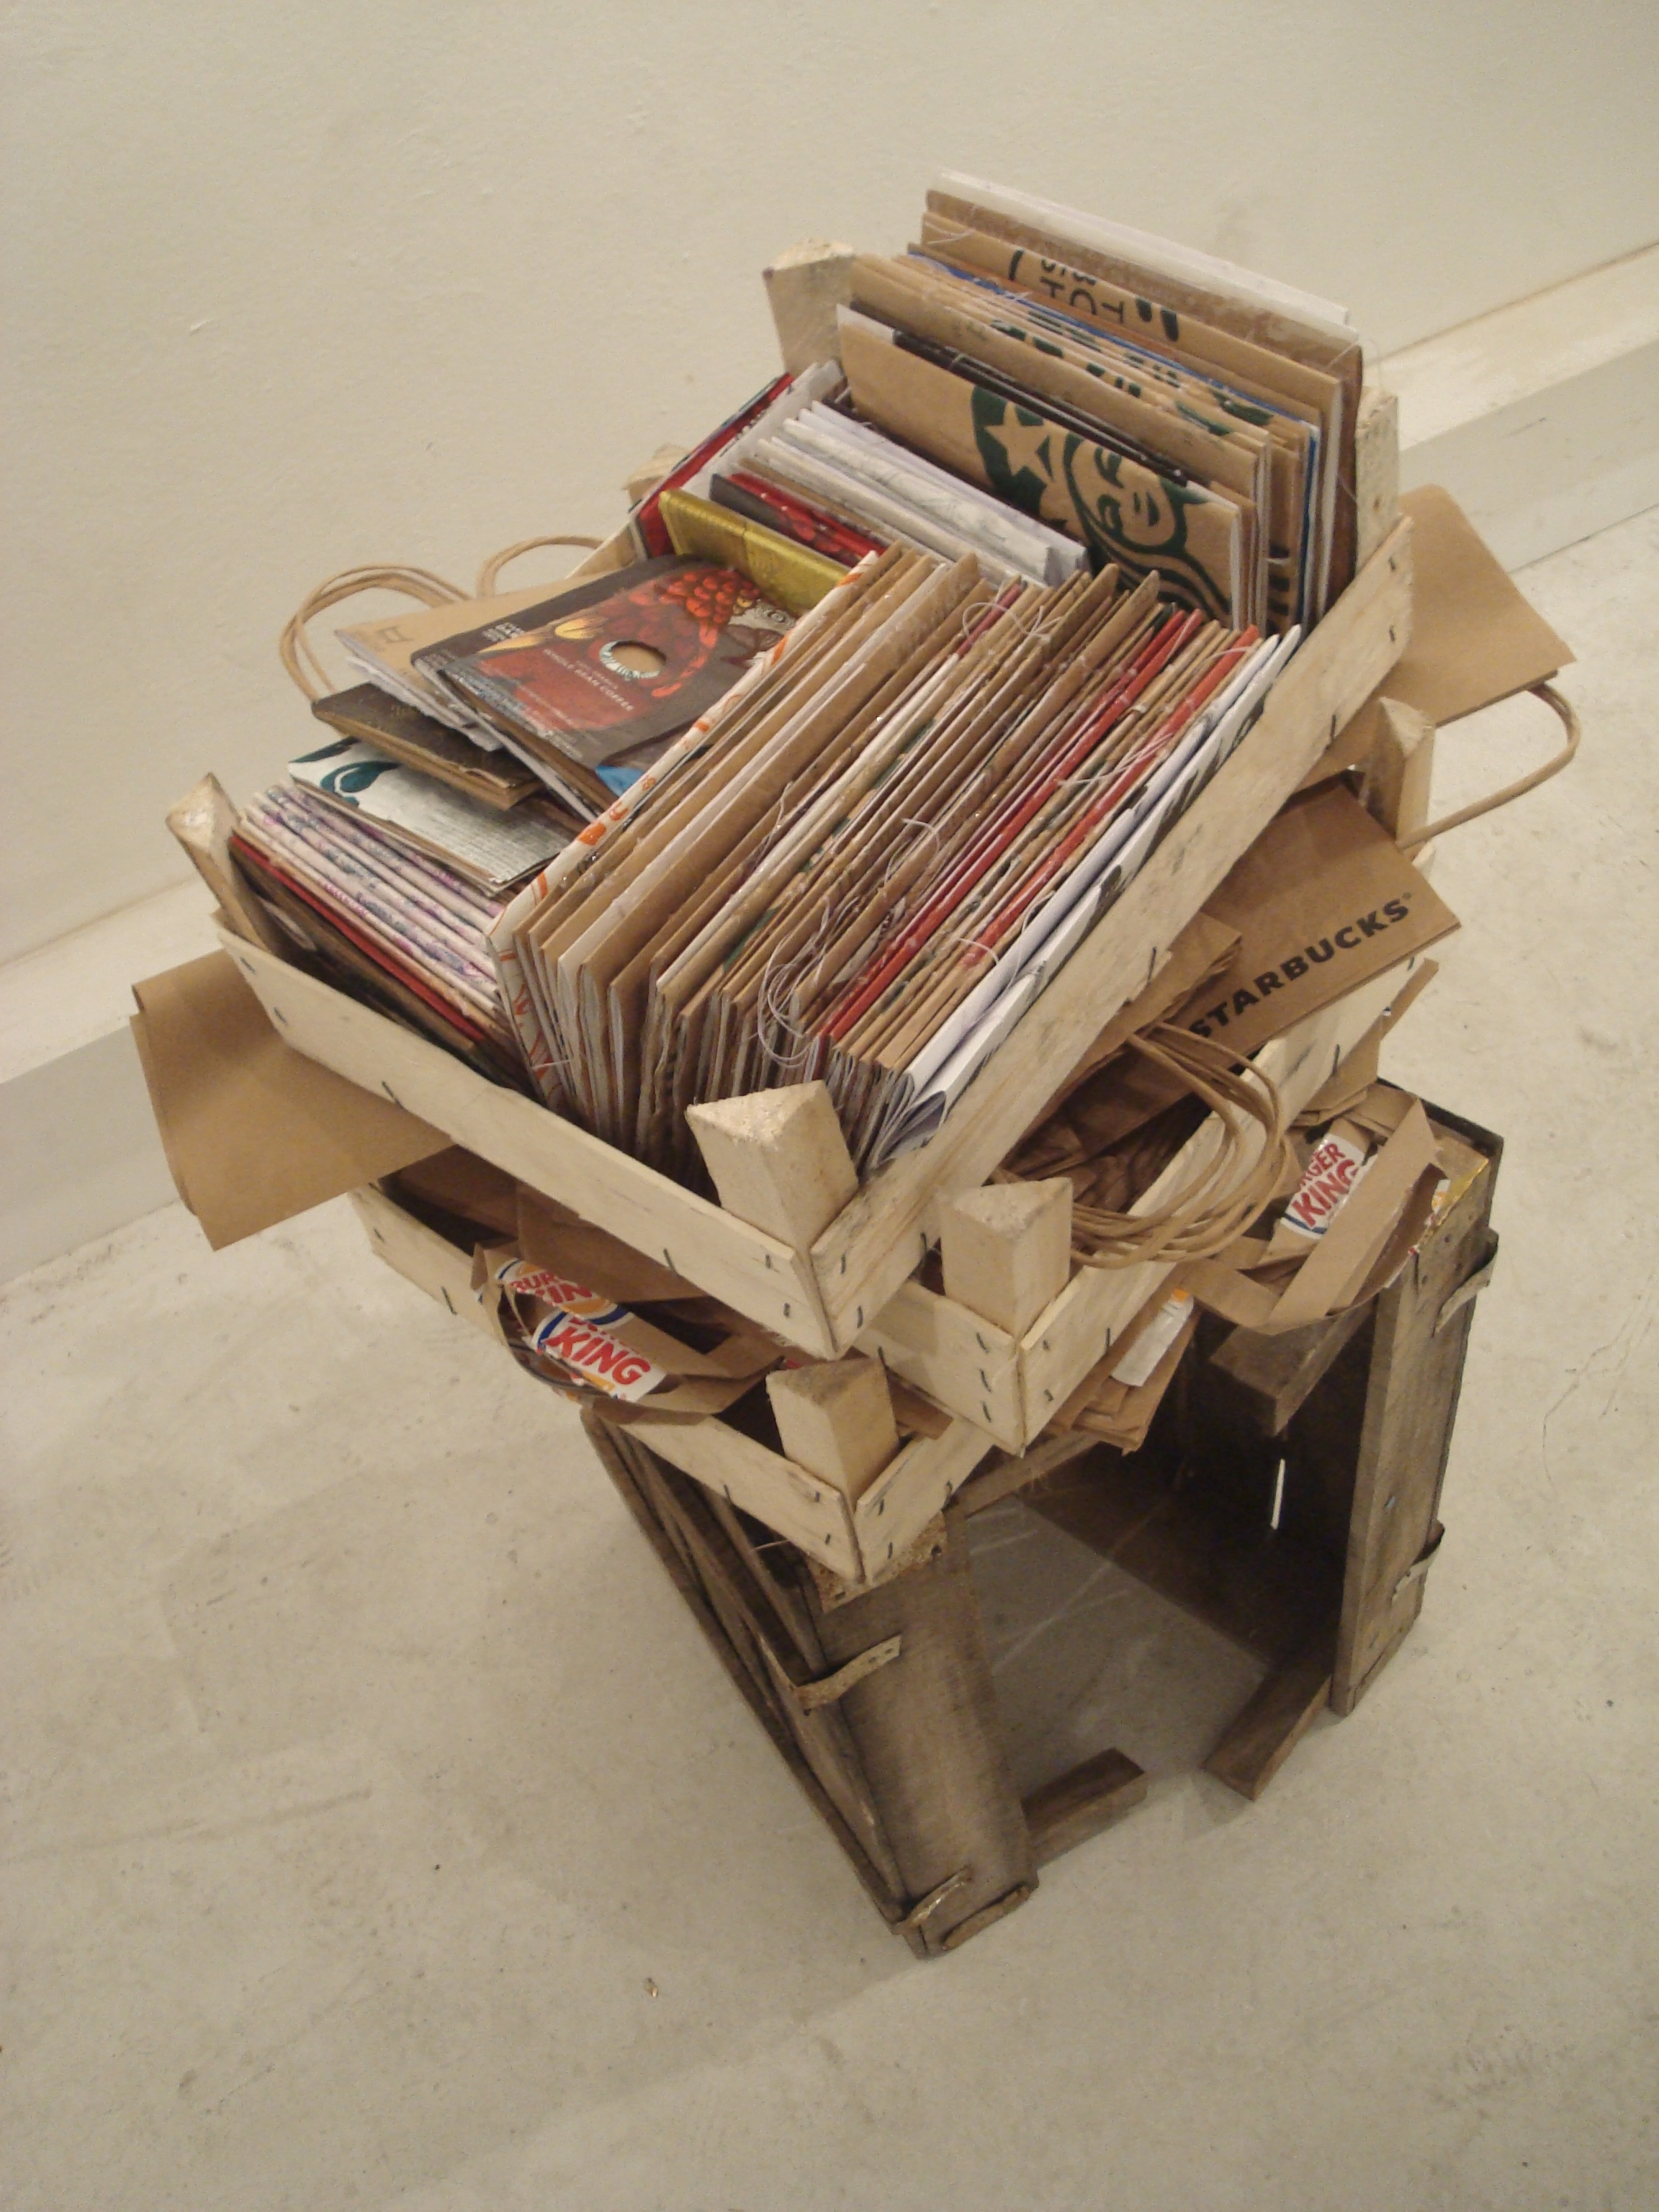
\includegraphics[width=\textwidth]{project_graphics/torun3.jpg}
  \end{subfigure}
  \hfill
  \begin{subfigure}[b]{0.48\textwidth}
    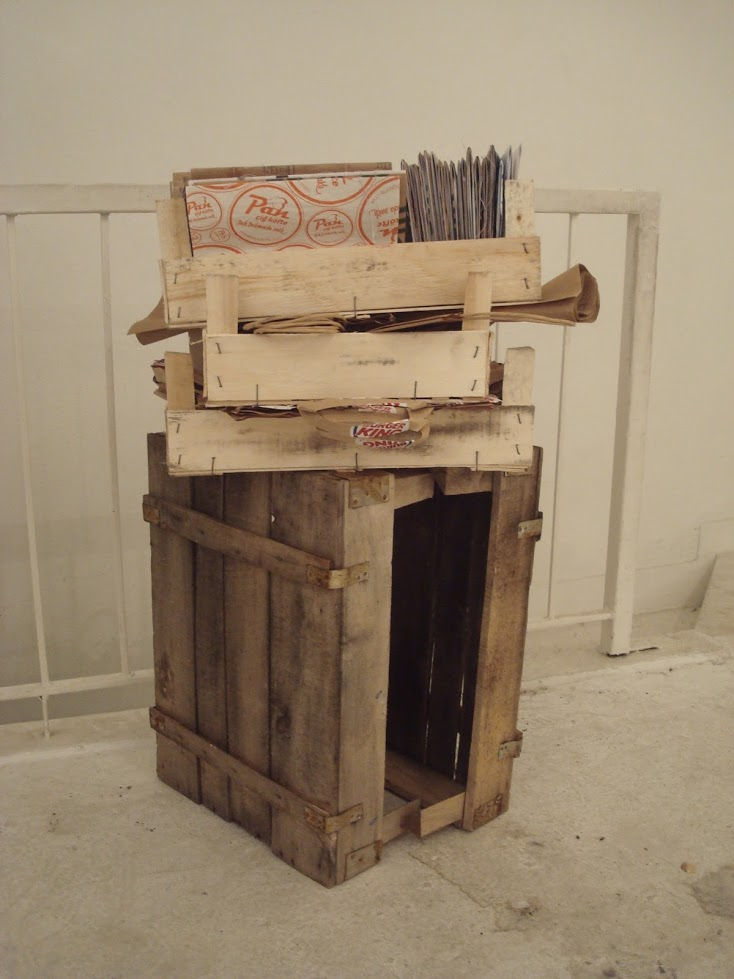
\includegraphics[width=\textwidth]{project_graphics/torun2.jpg}
  \end{subfigure}
  \caption{Sample placement at Torun}
  \label{fig:SamplePlacementAtTorun}
\end{figure}

Figure \ref{fig:SamplePlacementAtTorun} shows the example placements in Torun. The exhibition event is not held. It is only decided. These notebooks will not only be exhibited there, but also I will turn it to an workshop that I continue to produce notebooks and show people to how to do it. Maybe they will join me in the production of notebooks. They can bring their items and we can transform them all together. We can share our ideas and thoughts with each other. 



%****************************************
\subsection{Website}
Finding a new place to the discarded items is one of the main purposes of this project. Not only it finds a place in people’s life again, but also it finds another place in the digital space.

Mainly website displays the (hi)story of notebooks. It contains a section for how notebooks are produced and the story behind it. The purpose is to record the creative process and share with others. Revealing the process is significant to demystifiying the truth about the project. It makes it more clear that the object used here is actually transformed from something else. People can access to images and descriptions of notebooks. All the development process of the project will be revealed in this website. Will contain list of collected materials. 

Into the notebooks a sticker which contains qr code and short description with the address of website is pasted. People can able to reach more information through this reminders. 

\begin{figure}[h!]
  \centering
  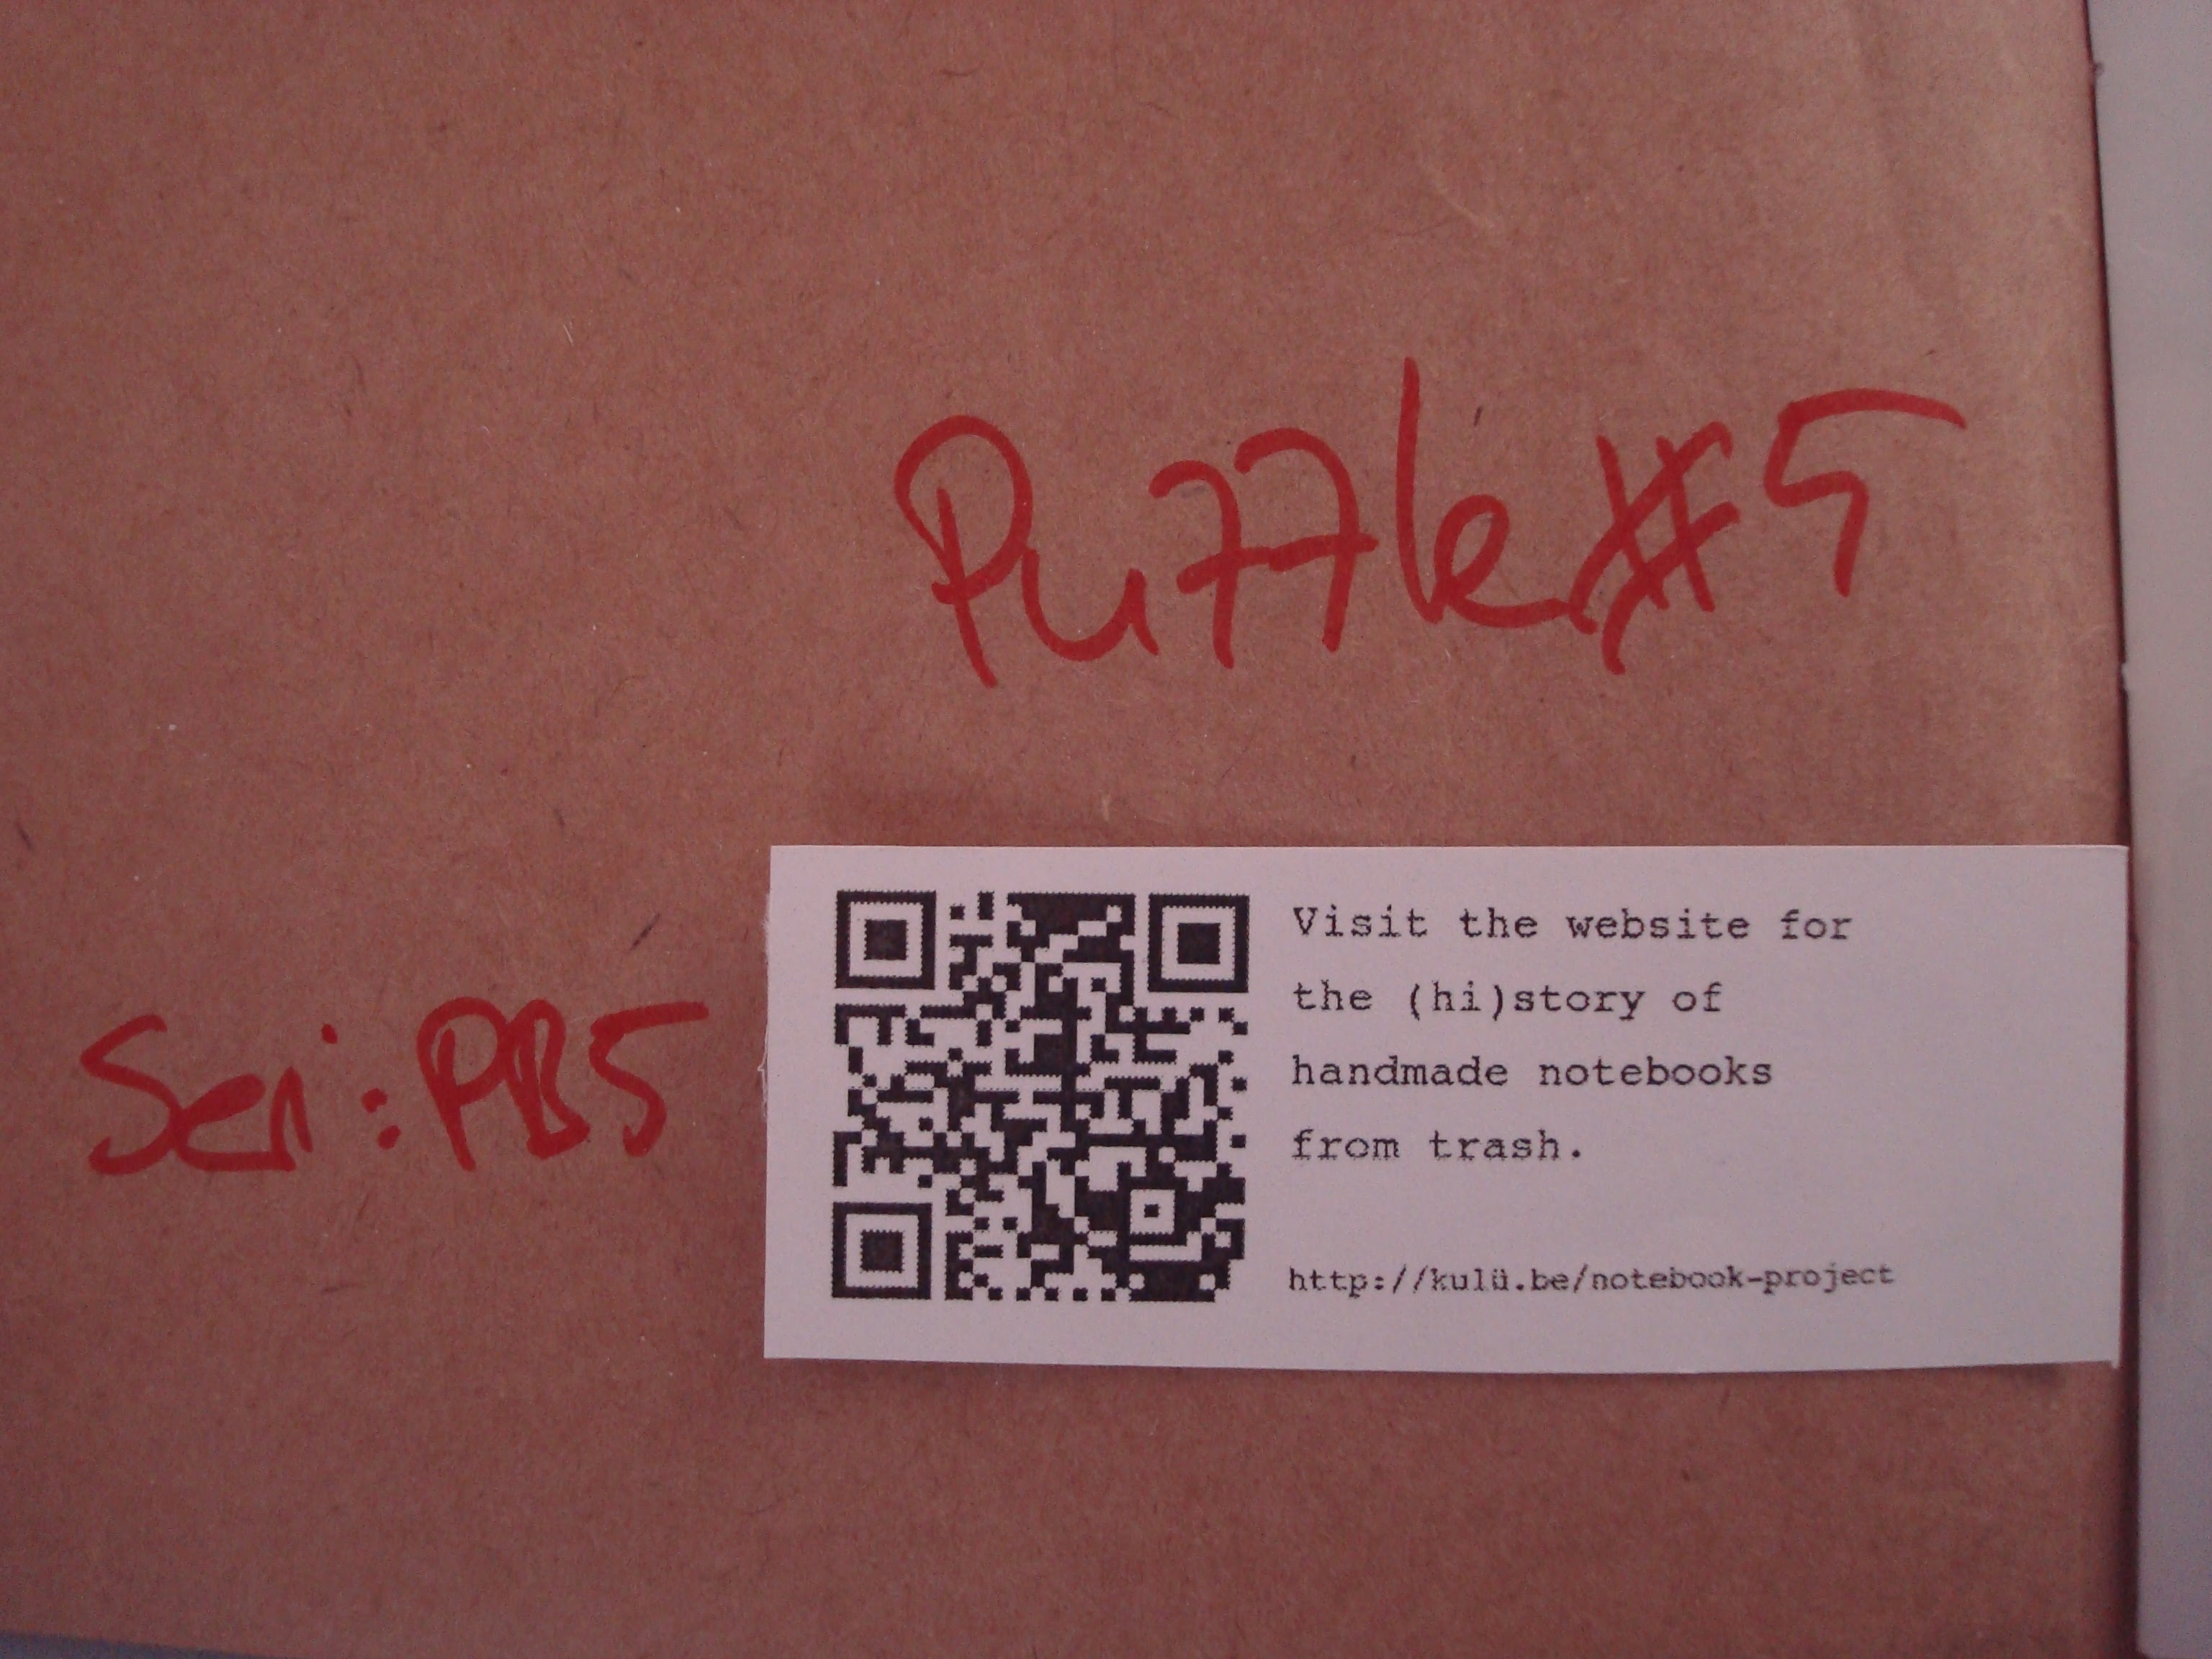
\includegraphics[width=1\textwidth]{project_graphics/qr_serial.jpg}
  \caption{Sample of QR code and notebook serial}
  \label{fig:QR}
\end{figure}

Website is a place to track the journey the notebooks. Transformation of it does not completed. It always continues. Therefore a website that anyone can reach and share their progress via website will show their evolution in time. Anyone can later discover how they turned to new things.

As I leave notebooks different places I do not have connection with people who take them. This website also will help to share peoples ideas about the notebooks.

Maybe it can be thought that there are different methods to accomplish recording and sharing the process. In a gallery on a single table or a room it can be succeed. However it like the idea that website can evolve by time as this work evolve in time. I think it matches perfectly. This is not a finished work, it continues and so the website also.

%SketchBook Project is also inspired me a lot especially in terms of website. This project provides a platform to people in order to share their works with other people. It contains lots of works from all over the world. Full of creativity and showcase of richness of people’s expressions on the small notebooks. My work can be considered as a sketch book project through trash. Sketches or only creative progress is not the only consideration. You can send your lecture notes.

Website can be accessible through this address: \url{http://kulu.be/notebook-project}. Domain name kulu.be belongs to me and project placed under a directory of it. Website is coded by me with the common and trusted open source libraries and frameworks. Its code also available at this address. Site is served from GitHub pages which provides free website hosting. Pages are generated by Jekyll which is a static website generator through it some repetitive works are can be easily automatized. 

Through the website people can be able to subscribe to the newsletter to get updates about the project. People can be able to add their comment to the website. How they are using their notebooks will be showed through it. Website will function as a platform to get into touch with people. From one point of view website can bee seen as a visitors book.

In the future all the discussions and research can be moved to the website that people can reach more information about the subject. This thesis and presentation will also be added to the website. 

All the progress up to now forms the core of the project. However it is not limited with it. The project will be continued after this thesis completed. New features will be added to the website. In the future it is planned that through the website people can be able to request to get notebooks. Thus notebooks become more accessible to the other people. Moreover notebooks done by others from trash can be added to the website. Beyond notebooks various objects transformed from trash can find a place in the website.

